% !TeX root = RJwrapper.tex
\title{Teaching Computers to See Patterns in Scatterplots with
Scagnostics}
\author{by Harriet Mason, Stuart Lee, Ursula Laa, and Dianne Cook}

\maketitle

\abstract{%
As the number of dimensions in a data set increases, the process of
visualising its structure and variable dependencies becomes more
tedious. Scagnostics (scatterplot diagnostics) are a set of numerical
measures describing visual features that can be used to identify
interesting and abnormal scatterplots, and give a sense of priority to
the variables we choose to visualise. A new set of scagnostics,
containing previously defined measures and newly created measures, are
implemented in the \texttt{cassowaryr} R package, which provides a
user-friendly method to apply scagnostics to data in R. After
implementing the scagnostics from the original defnitions we found that
some measures did not work as expected, and variations were developed.
The application of scagnostics is illustrated with four examples, sport
statistics, astrophysics, collections of time series and economic
indcators, that show they can be useful for exploratory data analysis,
identifying shape differences between groups, and as a summary tool for
the shape of multivariate data.
}

\hypertarget{introduction}{%
\section{Introduction}\label{introduction}}

Visualising our data is an important step in understanding the
underlying structure and cannot be ignored. Datasets like Anscombe's
quartet \citep{anscombe} or the Datasaurus Dozen \citep{datasaurpkg}
have been constructed such that each pairwise plot has the same summary
statistics but strikingly different visual features. These are designed
to illustrate the pitfalls of numerical summaries and the importance of
visualisation. Unfortunately visualising high dimensional data is often
difficult and requires a trade-off between the usefulness of the plots
and maintaining the structures of the original data. Due to limitations
in visualisation, it is often difficult to completely capture
relationships that involve more than two dimensions. Up to a moderate
number of variables, a scatter plot matrix (SPLOM) can be used to create
pairwise biplots of all variables, however, this solution quickly
becomes infeasible as the number of dimensions increases and the number
of plots in the SPLOM rises exponentially. There is a large amount of
research into visualising high dimensional data, most of which focuses
on some form of dimension reduction. Dimension reduction allows us to
manage high dimensional data, usually by selecting a subset of important
variables or performing a linear or non-linear transformation on the
variables in a way that captures the relevant information.
Unfortunately, these methods are not without their pitfalls. Linear
transformations are subject to crowding, that is, projections
concentrate data in the centre of the distribution making it difficult
to differentiate data points \citep{crowding}. Non-linear
transformations, such as t-distributed stochastic neighbour embedding
(t-SNE) \citep{tsne} often have complex parameterisations, and can break
the underlying global structure of the data, creating misleading
visualisations. There are solutions within these methods that can
somewhat mitigate these issues. To prevent crowding in a visualisation
of a linear transformation, a burning sage tour from the \texttt{tourr}
package proportionately zooms in more on the points in the centre of the
visualisation of than those of the outskirts \citep{burningsage}. To try
and maintain a sense of global structure in a non-linear transformation,
there are things like the \texttt{liminal} package which facilitates
linked brushing between linear and non-linear transformations
\citep{liminal}. These latter two methods of dimension reduction involve
dynamic graphics, which is not always easy to manage or even publish.

\emph{Scagnostics} are one possible alternative to variable
transformations, and can be particularly useful for producing a
hierarchy of variables, and capturing non-linear and unusual
relationships between variables. The term scagnostics was introduced by
John Tukey in 1982 (see pages 411, 427 and 433 of \citet{tukey}).
Tukey's suggestion to deal with the curse of dimensionality was to
filter out uninteresting variables using a cognostic. A cognostic is a
diagnostic that should be interpreted by a computer rather than a human
and those specific to scatter plots are called scagnostics. Instead of
trying to view every possible variable combination, the workload is
reduced by calculating a series of visual features, and only presenting
scatter plots that have interesting results on these feature
combinations. As scagnostics filter the plots, rather than transform the
data, they offer the benefit of allowing the user to view relationships
between the variables in their raw form. This means they are not subject
to the linear transformation issue of crowding, or the non-linear
transformation issue of misleading global structures. That being said,
only viewing select pairwise plots can leave our variable
interpretations without context. Viewing pairwise plots of the data with
another chart indicating their relative position in the scagnostic
distributions (found by computing scagnostics on every possible pairwise
plot in the data set), is one suggested solution \citep{scagexplorer},
but ultimately the lack of context remains a limitation in using
scagnostics alone as a high dimensional visualisation technique.

Scagnostics have found several applications since their initial
introduction by Tukey. \citet{hidscags} showed scagnostics to be a
valuable tool in finding hidden structures in biplots by combining them
with variable transformations (such as a log transform).
\citet{timeseer} used scagnostics to identify atypical sub-sequences
from multivariate time series data for further analysis. Also,
\citet{tourrpp} used them in the \texttt{tourr} projection pursuit to
find interesting low level projections of linear combinations of
variables.

Advancing Tukey's work, \citet{scag} defined computationally efficient
measures that were later refined by \citet{scagdist} which make up the
foundations of current scagnostics. In addition to these foundational
scagnostics, \citet{Grimm} introduced two additional association
scagnostics. These two association measures are also used in the
\texttt{tourr} projection pursuit \citep{tourrpp}.

There are two scagnostics packages that compute the measures defined by
\citet{scag}, \texttt{scagnostics} \citep{scagdist} and the archived
package \texttt{binostics} \citep{binostics}. Both packages are based on
the original C++ code written by \citet{scagdist} which is difficult to
read, debug, and extend upon. The two additional association measures
discussed by \citet{Grimm} were in the package \texttt{mbgraphic}, but
that has also been archived by CRAN. These gaps in accessibility
indicate that there is a need for a new implementation of scagnostics,
one that enables a better diagnosis of results and provides graphical
tools for examining these results.

The paper is organised as follows. The next section introduces the
scagnostics, explains how they are calculated, and develops several new
measures. This is followed by a summary of the implementation in the R
package, \texttt{cassowaryr}. Finally, the example section applies
scagnostics to four different data sets to illustrate their use in three
different tasks. The Australian Football League Women's (AFLW) data, and
a simulated binary black hole (BBH) merger event show the scagnostics
value as a tool in exploratory data analysis. The collection of time
series example, using macroeconomic and microeconomic data, illustrates
the scagnostics ability to differentiate groups by shape. The world bank
indicators (WBI) shows how scagnostics can be used to summarise the
shape of multivariate data.

\hypertarget{scagnostics}{%
\section{Scagnostics}\label{scagnostics}}

\hypertarget{building-blocks-for-the-graph-based-metrics}{%
\subsection{Building blocks for the graph-based
metrics}\label{building-blocks-for-the-graph-based-metrics}}

In order to capture the visual structure of the data, graph theory is
used to calculate most of the scagnostics. The pairwise scatter plot is
re-constructed as a graph with the data points as vertices and the edges
are calculated using Delaunay triangulation. In the package, this
calculation is done using the alphahull package \citep{alphahull} to
construct an object called a \texttt{scree}. All the graph based
scagnostics use the scree in their calculations, the association based
scagnostics only use the raw data. The \texttt{scree} object is then
used to construct the three key structures on which the scagnostics are
based; the convex hull, alpha hull and minimum-spanning tree (MST)
(Figure \ref{fig:building-blocks2}).

\begin{itemize}
\item
  \textbf{Convex hull:} The outside vertices of the graph, connected to
  make a convex polygon that contains all points. It is constructed
  using the tripack package \citep{tripack}.
\item
  \textbf{Alpha hull:} A collection of boundaries that contain all the
  points in the graph. Unlike the convex hull, it does not need to be
  convex. It is calculated using the alpha hull package
  \citep{alphahull}.
\item
  \textbf{MST:} The minimum spanning tree (MST) is the shortest distance
  of branches that can be used to connect all the points. It is
  calculated from using the igraph package \citep{igraph}.
\end{itemize}

\begin{Schunk}
\begin{figure}
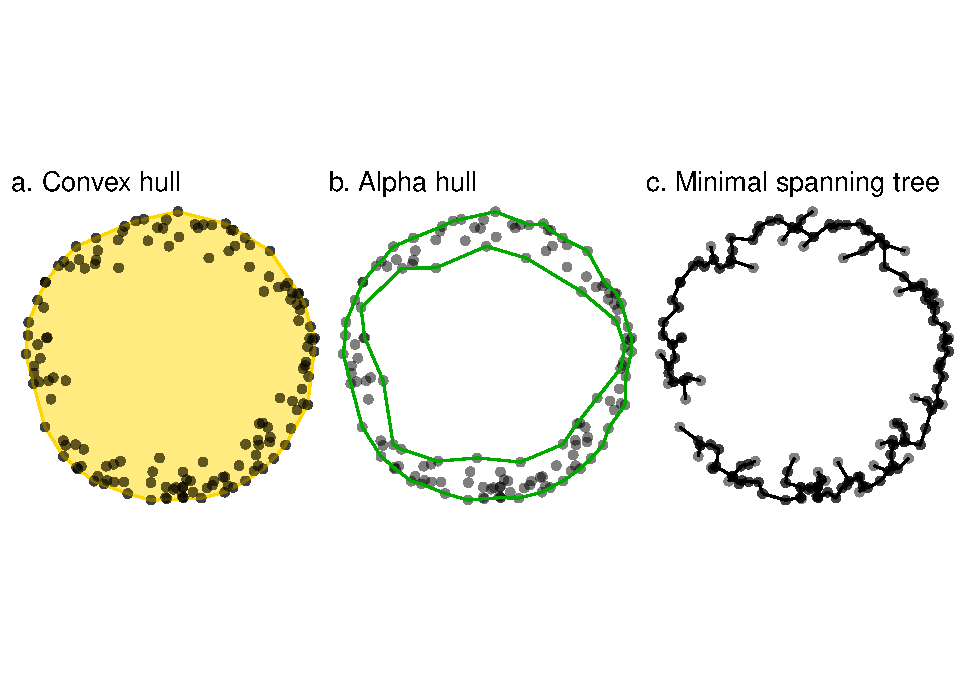
\includegraphics[width=1\linewidth]{mason-lee-laa-cook_files/figure-latex/building-blocks2-1} \caption[The building blocks for graph-based scagnostics]{The building blocks for graph-based scagnostics: (a) convex hull, (b) alpha hull and (c) minimal spanning tree. The convex hull is a convex shell around all the data points. The alpha hull contains all the points but allows concavities better capturing some shapes, but it needs tuning. The minimal spanning tree connects all points once, and has a single chain connecting central points.}\label{fig:building-blocks2}
\end{figure}
\end{Schunk}

The nine scagnostics defined by \citet{scagdist} are detailed below with
an explanation and a formula. They were all constructed to range
{[}0,1{]}, and later scagnostics have maintained this scale. To give
further understanding in how these measures work, the scagnostics
\emph{skinny}, \emph{outlying}, and \emph{clumpy} are given an
additional visual explanation in Figure \ref{fig:scagdrawn}. We will let
\(A=\) alpha hull, \(C=\) convex hull, \(M\) = minimum spanning tree,
and \(s=\) the scagnostic measure. Since some of the measures have a
sample size dependence, \(\omega=0.7 + \frac{0.3}{1 + \frac{n}{500}}\)
is a parameter used to mitigate sample size bias where \(n\) is the
number of points \citep{scagdist}.

Before any of the scagnostics are calculated, outlying points are
removed. Outliers are defined as any point whose adjacent edges in the
MST have edges larger \(q_{75} + 1.5(q_{75} - q_{25})\), where \(q_i\)
refers to the i\(^{th}\) percentile of the sorted edge lengths of the
MST.

\begin{Schunk}
\begin{figure}
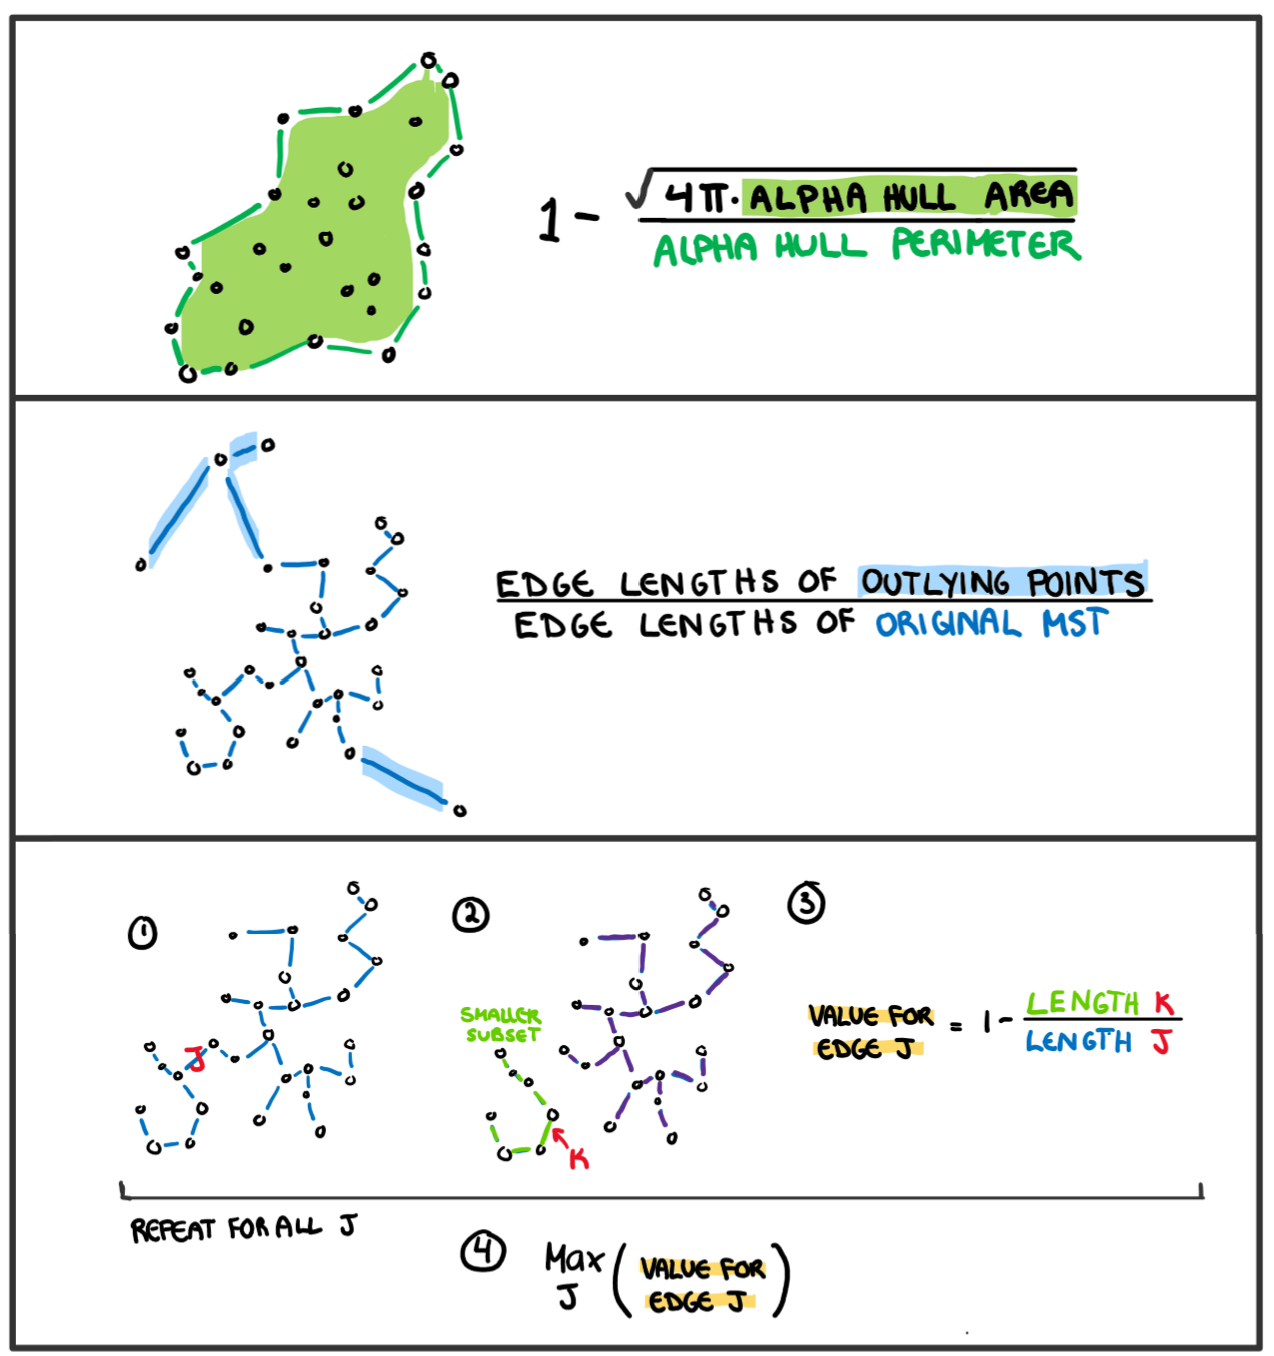
\includegraphics[width=1\linewidth]{figures/drawnmeasures} \caption[ An visualisation of the calculation used to compute the skinny (top), outlying (middle), and clumpy (bottom) scagnostics]{ An visualisation of the calculation used to compute the skinny (top), outlying (middle), and clumpy (bottom) scagnostics. These three measure definitions are quite distinct, and each illustrates a unique method of capturing a visual feature in a scatter plot.}\label{fig:scagdrawn}
\end{figure}
\end{Schunk}

\hypertarget{graph-based-scagnostics}{%
\subsection{Graph-based scagnostics}\label{graph-based-scagnostics}}

\begin{itemize}
\tightlist
\item
  \textbf{Convex:} Measure of how convex the shape of the data is.
  Computed as the ratio between the area of the alpha hull (\(A\)) and
  convex hull (\(C\)). Unlike the other scagnostic measures, a high
  value on convex does not correlate to an interesting scatter plot,
  rather it usually indicates a lack of relationship between the two
  variables.
\end{itemize}

\[s_{convex}=\frac{\mbox{area}(A)}{\mbox{area}(C)}\]

\begin{itemize}
\tightlist
\item
  \textbf{Skinny:} A measure of how ``thin'' the shape of the data is.
  It is calculated as the ratio between the area and perimeter of the
  alpha hull (\(A\)) with some normalisation such that 0 correspond to a
  perfect circle and values close to 1 indicate a skinny polygon.
\end{itemize}

\[s_{skinny}= 1-\frac{\sqrt{4\pi \mbox{ area}(A)}}{\mbox{perimeter}(A)}\]

\begin{itemize}
\tightlist
\item
  \textbf{Outlying:} A measure of proportion and severity of outliers in
  dataset. Calculated by comparing the edge lengths of the outlying
  points in the MST (\(M_{outliers}\)) with the length of the entire MST
  (\(M\)).
\end{itemize}

\[s_{outlying}=\frac{\mbox{length}(M_{outliers})}{\mbox{length}(M)}\]

\begin{itemize}
\tightlist
\item
  \textbf{Stringy:} This measure identifies a ``stringy'' shape with no
  branches, such as a thin line of data. It is calculated by comparing
  the number of vertices of degree two (\(V^{(2)}\)) with the total
  number of vertices (\(V\)), dropping those of degree one
  (\(V^{(1)}\)).
\end{itemize}

\[s_{stringy} = \frac{|V^{(2)}|}{|V|-|V^{(1)}|}\]

\begin{itemize}
\tightlist
\item
  \textbf{Skewed:} A measure of skewness in the edge lengths of the MST
  (not in the distribution of the data). It is calculated as the ratio
  between the 90th to 50th percentile range and the central 80th
  interpercentile range.
\end{itemize}

\[s_{skewed} = 1-\omega\left(1-\frac{q_{90}-{q_{50}}}{q_{90}-q_{10}}\right)\]

\begin{itemize}
\tightlist
\item
  \textbf{Sparse:} Identifies if the data is sporadically located on the
  plane. Calculated as the 90th percentile of MST edge lengths.
\end{itemize}

\[s_{sparse}= \omega q_{90}\]

\begin{itemize}
\tightlist
\item
  \textbf{Clumpy:} This measure is used to detect clustering and is
  calculated through an iterative process. First an edge J is selected
  and removed from the MST. From the two spanning trees that are created
  by this break, we select the largest edge from the smaller tree
  (\(K\)). The length of this edge (\(K\)) is compared to the removed
  edge (\(J\)) giving a clumpy measure for this edge. This process is
  repeated for every edge in the MST and the final clumpy measure is the
  maximum of this value over all edges.
\end{itemize}

\[\max_{j}\left[ 1-\frac{\max_{k}[\mbox{length}(e_k)]}{\mbox{length}(e_j)}\right]\]

\begin{itemize}
\tightlist
\item
  \textbf{Striated:} This measure identifies features such as
  discreteness by finding parallel lines. Calculated by counting the
  proportion of vertices with only two edges that have an inner angle
  approximately between 135 and 220 degrees.
\end{itemize}

\[\frac1{|V|}\sum_{v \in V^{2}}I(\cos\theta_{e(v,a)e(v,b)}<-0.75)\]

\hypertarget{association-based-scagnostics}{%
\subsection{Association-based
scagnostics}\label{association-based-scagnostics}}

\begin{itemize}
\tightlist
\item
  \textbf{Monotonic:} Checks if the data has an increasing or decreasing
  trend. Calculated as the Spearman correlation coefficient, i.e.~the
  Pearson correlation between the ranks of x and y.
\end{itemize}

\[s_{monotonic} = r^2_{Spearman}\]

The are two additional association scagnostics discussed by
\citet{Grimm} which are also implemented into the \texttt{cassowaryr}
package.

\begin{itemize}
\tightlist
\item
  \textbf{Splines:} Measures the functional non-linear dependence by
  fitting a penalised splines model on \(X\) using \(Y\), and on \(Y\)
  using \(X\). The variance of the residuals are scaled down by the axis
  so they are comparable, and finally the maximum is taken. Therefore
  the value will be closer to 1 if either relationship can be decently
  explained by a splines model.
\end{itemize}

\[s_{splines}=\max_{i\in x,y}\left[ 1-\frac{\mbox{Var}(\mbox{Residuals}_{model~i=.})}{\mbox{Var}(i)}\right] \]

\begin{itemize}
\tightlist
\item
  \textbf{Dcor:} A measure of non-linear dependence which is 0 if and
  only if the two variables are independent. Computed using an ANOVA
  like calculation on the pairwise distances between observations.
\end{itemize}

\[s_{dcor}= \sqrt{\frac{\mathcal{V}(X,Y)}{\mathcal{V}(X,X)\mathcal{V}(Y,Y)}}\]\\
where \[\mathcal{V}
(X,Y)=\frac{1}{n^2}\sum_{k=1}^n\sum_{l=1}^nA_{kl}B_{kl}\]\\
where \[A_{kl}=a_{kl}-\bar{a}_{k.}-\bar{a}_{.j}-\bar{a}_{..}\]
\[B_{kl}=b_{kl}-\bar{b}_{k.}-\bar{b}_{.j}-\bar{b}_{..}\]

\hypertarget{checking-the-scagnostics-calculations}{%
\subsection{Checking the scagnostics
calculations}\label{checking-the-scagnostics-calculations}}

To test the packages ability to differentiate plots, we have created a
dataset called \emph{features} (Figure \ref{fig:features-plot}), that
contains a series of interesting and unique scatter plots. These scatter
plots each typify a certain visual feature. These include a
deterministic relationship, discreteness in variables, or clustering,
and scagnostics are used to order these scatter plots based on the
prevalence of these various visual features.

\begin{Schunk}
\begin{figure}
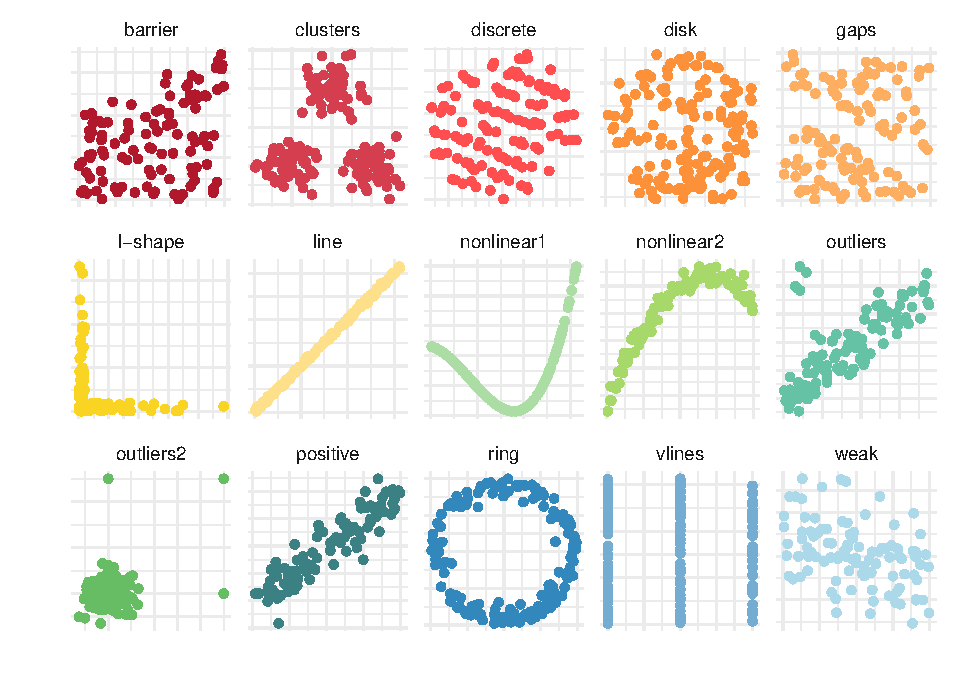
\includegraphics[width=1\linewidth]{mason-lee-laa-cook_files/figure-latex/features-plot-1} \caption[The scatter plots of the features dataset]{The scatter plots of the features dataset. These scatter plots were designed to each represent a distinct visual feature, for example the ring scatter plot is a hollow version of disk. The scagnostics need to be able to differentiate these plots.}\label{fig:features-plot}
\end{figure}
\end{Schunk}

Figure \ref{fig:visual-table} shows scatter plots from the features data
aligned on a 0 to 1 scale for each scagnostic. This visualisation
displays a low, high, and moderate value for each scagnostic, and is
useful to see how the scagnostics order data that typifies their visual
feature. This plot gives us an idea of the issues some of the
scagnostics face in their current state. The scagnostics are supposed to
range from 0 to 1 however in some cases the values are so compressed
that a moderate value would not fit, indicating that the scagnostics do
not quite work as intended. The scagnostics based upon the convex hull
(i.e.~skinny and convex) work fine, as do the association measures such
as monotonic, dcor and splines. The main issues come from the measures
based on the MST. We can see in the figure that the sparse, stringy,
skewed, and clumpy are each concentrated on a small portion of 0 to 1
number line. In addition to this, clumpy does not correctly order the
scatter plots according to human intuition, and while it is not visible
here, striated also struggles with a correct ordering. We suspect the
reason for these warped distributions is the removal of binning as a
preliminary step in calculating the scagnostics. The removal of binning
allows for a large number of arbitrarily small edges, which upon testing
was found to be the cause of a lot of these issues. A summary of how
binning warped each MST scagnostic is provided in Table
\ref{tab:scagissues-tb-pdf}. We wanted the package to have binning as an
optional method, considering choices in binning can lead to bias as
noted in \citet{scagdist} or unreproducible results as noted in
\citet{robust}. Therefore the scagnostics were assessed without binning.

\begin{Schunk}
\begin{table}

\caption{\label{tab:scagissues-tb-pdf}Summary of MST scagnostic issues.}
\centering
\begin{tabular}[t]{l>{\raggedright\arraybackslash}p{12cm}}
\toprule
Scagnostic & Issues\\
\midrule
Striated & The striated measure can identify the specific case of one discrete variable and one continuous variable but cannot identify two discrete variables. Since by definition it is a subset of the stringy measure, they are highly correlated, and often plots that striated identifies as interesting have already been identified by stringy.\\
Sparse & While sparse does seem to identify spread out distributions, it rarely returns a value higher than 0.1. The removal of binning means the number of values that can cluster on one portion of the plane is infinite. Even if the rest of the scatter plot is sparse, this one cluster will arbitrarily keep the sparse value low. With a large number of observations on two continuous variables, this is unavoidable, which also means the measure does not have consistancy.\\
Skewed & This measure can identify skewed edge lengths, such as the L shape in the visual table, however its value rarely drop below 0.5 or rise above 0.8. Skewed seems to suffers from a similar issue to sparse reguarding binning.\\
Outlying & By definition an outlier must have all its adjacent edges in the MST above the outlying threshold. This means two or more observations that are close together but away from the main mass of data will not be identified as outliers, which does not align with human intuition. Even if we change the measure such that only one edge needs to be above the outlying threshold, it would only remove a single point. The measure also struggles with distributions that have an increasing variance due to the removal of binning. If the number of points close to the centre of the cluster is large enough, outlying identifies the spread out points to be outliers and returns a large value, once again going against human intuition.\\
Stringy & This measure rarely drops below 0.5 even on data generated from a random normal distribution (which should intuitively return a 0). Unlike the other scagnostics on this list, stringy does not depend upon the edge lengths of the MST, so it is hard to say if this issue stems from binning. That being said, it was not reported in the binned version of the scagnostics, and so is likely a result of binning.\\
\addlinespace
Clumpy & With the removal of binning, clumpy does not identify a long edge connected to a short edge, but rather identifies any edge connected to an arbitrarily small edge. This means the clumpy measure rarely drops below 0.9, and also does not correctly order the edges.\\
\bottomrule
\end{tabular}
\end{table}

\end{Schunk}

While we mentioned some issues in the distributions of the scagnostics,
in that they do not seem to range from 0 to 1, these measures will not
be adjusted. Testing the distribution and consistency of the binned
scagnostics was done previously by \citet{scagdist}, however it was
completed as a separate research project to the creating of the original
scagnostics. Assessing the scagnostic distributions is a considerable
task, that would require checking the measures on a range of data from
multiple disciplines to ensure we are finding the true ``global''
distributions. This task that is beyond the scope of this research, and
we will assume that the scagnostics range uniformly from 0 to 1 and only
adjust those measures that provide an incorrect ordering.

\begin{Schunk}
\begin{figure}
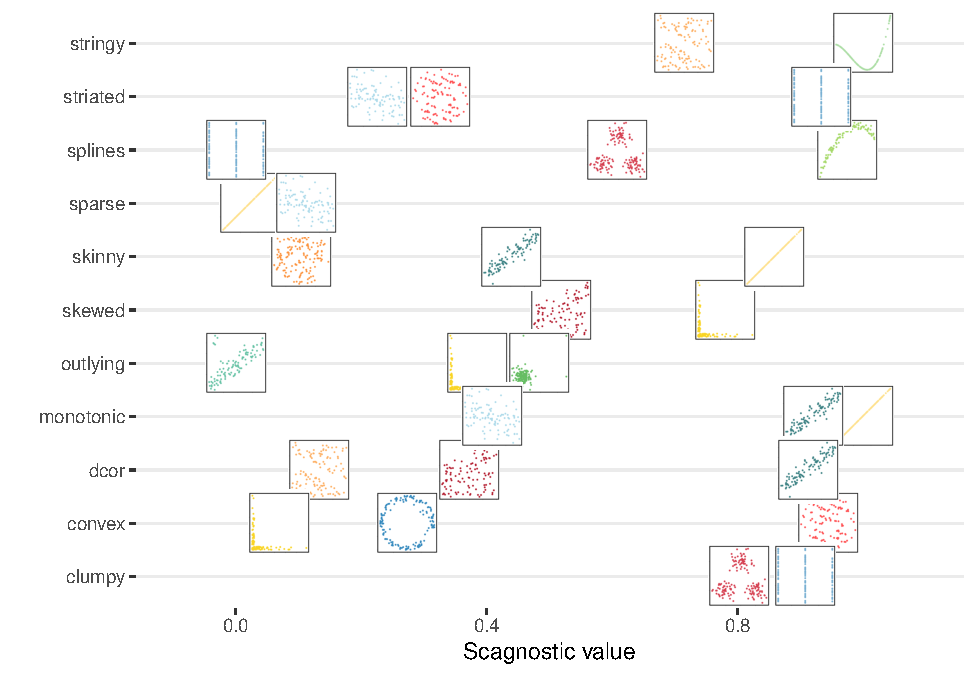
\includegraphics[width=1\linewidth]{mason-lee-laa-cook_files/figure-latex/visual-table-1} \caption[A visual table that displays a selection of scagnostics computed on the features data]{A visual table that displays a selection of scagnostics computed on the features data. The rows correspond to different scagnostics and the horizontal axis is the calculated value on a range of 0-1. Thumbnail plots of variable pairs are placed at their scagnostic value, and indicate the type of structure that would produce high or low or medium values. Some scagnostics, e.g. clumpy, need adjustment as they do not correctly order the scagnostics, or range from 0 to 1. Other measures, such as splines work without any changes to their definition.}\label{fig:visual-table}
\end{figure}
\end{Schunk}

\hypertarget{the-adjusted-scagnostics-measures}{%
\subsubsection{The adjusted scagnostics
measures}\label{the-adjusted-scagnostics-measures}}

\hypertarget{striated-adjusted}{%
\paragraph{Striated adjusted}\label{striated-adjusted}}

The issues that need to be addressed with the new striated measure are:

\begin{enumerate}
\def\labelenumi{\arabic{enumi}.}
\tightlist
\item
  By only counting vertices with 2 edges, the set of vertices counted in
  this measure are a subset of those counted in stringy, thus the two
  measures are highly correlated.
\item
  In order for the vertex to be counted, the angle between the edges
  needs to be approximately 135 to 220 degrees. The relaxed bounds
  around 180 degrees seems to have been to give an allowance for points
  moving due to binning. With the removal of binning this leeway is
  unnecessary and many plots that are not discrete are identified as
  such.
\end{enumerate}

To account for these two issues the striated adjusted measure considers
all vertices (not just those with two adjacent edges), and makes the
measure strict around the 180 and 90 degree angles. With this we can see
the improvements on the measure in Figure \ref{fig:striated-vtable}.

\begin{Schunk}
\begin{figure}
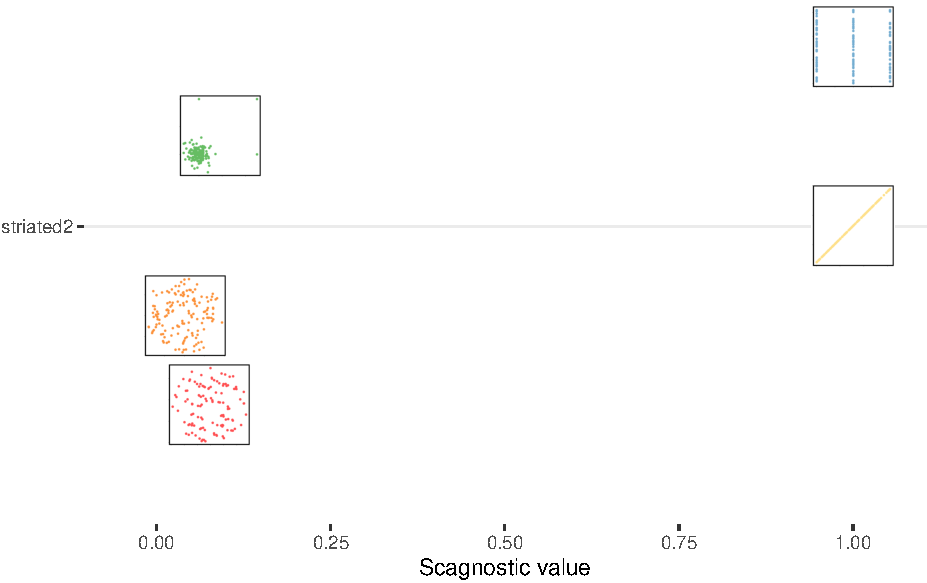
\includegraphics[width=1\linewidth]{mason-lee-laa-cook_files/figure-latex/striated-vtable-1} \caption[Using a visual table to compare the striated and it's adjusted counterpart, striated2 allows us to visualise the difference in the measures]{Using a visual table to compare the striated and it's adjusted counterpart, striated2 allows us to visualise the difference in the measures. While the functions may seem similar at a glance, striated2 has a stricter version of discreteness, hence why line and vlines have the same result and plots with no discreteness score a 0.}\label{fig:striated-vtable}
\end{figure}
\end{Schunk}

Figure \ref{fig:striated-vtable} shows that while these two measures may
seem similar at a glance, there are a few minor differences that make
striated2 an improvement upon the original striated scagnostic. First of
all, the perfect 1 value on striated goes to the \emph{line} scatter
plot. While this does fulfill the definition, it is not what the measure
is supposed to be looking for, rather, it is supposed to be identifying
the \emph{vlines} scatter plot. Since striated does not count the right
angles that go between the vertical lines, a truly striated plot will
never get a full 1 on this measure, striated2 fixes this. After that
there is a large gap in both measures because none of the other scatter
plots have a strictly discrete measure on the x or y axis. Additionally,
while it is not visible in Figure \ref{fig:striated-vtable}, striated2
can identify discreteness when it appears in both axis with a small
number of observation, an additional version of discreteness that the
original striated struggles to identify. Both version of striated are
unable to recognise the \emph{discrete} plot, which is a noisy and
rotated version of discreteness, so there is still room for improvement
on this measure.

\hypertarget{clumpy-adjusted}{%
\paragraph{Clumpy adjusted}\label{clumpy-adjusted}}

The issues that need to be addressed with the new clumpy measure are:

\begin{enumerate}
\def\labelenumi{\arabic{enumi}.}
\tightlist
\item
  It needs to consider more than 1 edge in its final measure to make it
  more robust
\item
  The impact of the ratio between the long and short edges need to be
  weighted by the size of their clusters so the measure does not simply
  identify outliers
\item
  It should not consider vertices that's adjacent angles form a straight
  line (to avoid identifying plots already identifies as interesting by
  striated)
\end{enumerate}

Before creating a new clumpy measure, we looked into applying a
different adjustment defined by \citet{robust} that is a robust version
of the original clumpy measure. This version of clumpy has been included
in the package as \texttt{clumpy\_r} however it is not included as an
option in the higher level functions such as \texttt{calc\_scags()}
because its computation time is too long. The robust clumpy measure
builds multiple clusters, each having their own clumpy value, and then
returns the weighted sum, where each value is weighted by the number of
observations in that cluster. This version of clumpy has a more uniform
distribution between 0 and 1 and is more robust to outliers, however it
still does a poor job of ordering plots without the assistance of
binning. Since this scagnostic cannot be used in large scale scagnostic
calculations (such as those done on every pairwise combination of
variables as is intended by the package) and it maintains the ordering
issue from the original measure, it is not discussed here.

Therefore in order to fix the issues in the clumpy measure described
above, we designed an adjusted clumpy measure, called clumpy2, and it is
calculated as follows:

\begin{enumerate}
\def\labelenumi{\arabic{enumi}.}
\tightlist
\item
  Sort the edges in the MST
\item
  Calculate the difference between adjacent edges in this ordering, and
  find the index of the maximum. This maximum difference should indicate
  the jump from between cluster edges and inter-cluster edges.
\item
  Remove the between cluster edges from the MST and build clusters using
  the remaining edges
\item
  For each between cluster edge, take the smaller of the two clusters it
  is connected to and take its median edge length. The clumpy value for
  that edge is the ratio between the large and small edge lengths
  \(\frac{\mbox{edge}_{small}}{\mbox{edge}_{large}}\), with a two
  multiplicative penalties, one for uneven clusters
  (\(\sqrt\frac{2\times n_{small}}{n_{small}+n_{big}}\)) and one for
  ``stringy'' scatter plots (\(1-s_{stringy}\)) that is only applied if
  the stringy value is higher than 0.95, to reduce the arbitrarily large
  clumpy scores that come from striated plots.
\item
  Take the mean clumpy value for each between cluster edge, if it is
  below 1 it is beneath the threshold that is considered clumpy, and the
  value is adjusted to 1.
\item
  clumpy2 returns \(1-\frac{1}{\mbox{mean}(clumpy_i)}\)
\end{enumerate}

With this calculation, we generate the clumpy2 measure which is compared
to the original clumpy measure in the Figure \ref{fig:clumpy-vtable}.
Here we can see the improvements made on the clumpy measure in both
distribution from 0 to 1 and ordering. The measure is more spread out,
and so values range more accurately from 0 to 1. More importantly the
measure does a better job of ordering the scatter plots. On the original
clumpy measure the \emph{clusters} scatter plot was next to last, on the
clumpy2 measure \emph{clusters} is is identified as the most clumpy
scatter plot. Clumpy2 also has a penalty for uneven clusters (to avoid
being large due to a small collection of outliers) and clusters created
arbitrarily due to discreteness (such as \emph{vlines}) in order to
better align with the human interpretation of clumpy. With these
changes, the stronger performance of clumpy2 is apparent in this visual
table.

\begin{Schunk}
\begin{figure}
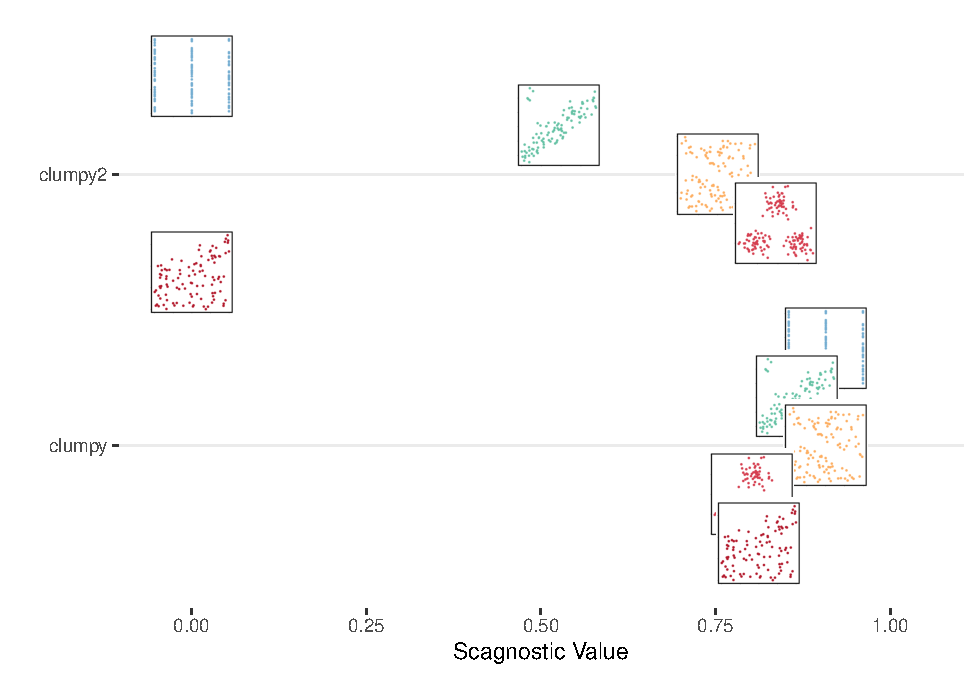
\includegraphics[width=1\linewidth]{mason-lee-laa-cook_files/figure-latex/clumpy-vtable-1} \caption[A visual table comparing the scagnostic values of clumpy and clumpy2]{A visual table comparing the scagnostic values of clumpy and clumpy2. We can see the clusters plot is next to last in the ordering of the original clumpy measure, but first in clumpy2. It is clear that clumpy2 achieves a more ballanced distribution and more intuitive plot ordering.}\label{fig:clumpy-vtable}
\end{figure}
\end{Schunk}

\hypertarget{implementation}{%
\section{Implementation}\label{implementation}}

\hypertarget{installation}{%
\subsection{Installation}\label{installation}}

The package can be installed from CRAN using

\begin{quote}
\texttt{install.packages("cassowaryr")}
\end{quote}

and from GitHub using

\begin{quote}
\texttt{remotes::install\_github("numbats/cassowaryr")}
\end{quote}

to install the development version.

\hypertarget{web-site}{%
\subsection{Web site}\label{web-site}}

More documentation of the package can be found at the web site
\url{https://numbats.github.io/cassowaryr/}.

\hypertarget{data-sets}{%
\subsection{Data sets}\label{data-sets}}

The \texttt{cassowaryr} package comes with several data sets that load
with the package. These are described in Table
\ref{tab:datasets-tb-pdf}.

\begin{Schunk}
\begin{table}

\caption{\label{tab:datasets-tb-pdf}Cassowaryr data sets}
\centering
\begin{tabular}[t]{>{\raggedright\arraybackslash}p{4cm}>{\raggedright\arraybackslash}p{8cm}}
\toprule
data & explanation\\
\midrule
features & Simulated data with special features.\\
anscombe\_tidy & Data from Anscombes famous example in tidy format.\\
datasaurus\_dozen & Datasaurus Dozen data in a long tidy format.\\
datasaurus\_dozen\_wide & Datasaurus Dozen Data in a wide tidy format.\\
numbat & A toy data set with a numbat shape hidden among noise variables.\\
\addlinespace
pk & Parkinsons data from UCI machine learning archive.\\
\bottomrule
\end{tabular}
\end{table}

\end{Schunk}

\hypertarget{functions}{%
\subsection{Functions}\label{functions}}

\hypertarget{scagnostics-functions}{%
\subsubsection{Scagnostics functions}\label{scagnostics-functions}}

The scagnostics functions functions either directly calculate each
scagnostic measure, or are involved in the process of calculating a
scagnostic measure (such as making the hull objects). These functions
are low level functions, and while they are exported by the package,
they are not the intended method of calculating scagnostics as they
perform no outlier removal, however they are still an option for users
if they wish. In some cases, such as \texttt{sc\_clumpy\_r} for clumpy
robust, they are the only method to calculate that scagnostic. Table
\ref{tab:scagfuncs-tb-pdf} outlines these functions.

\begin{Schunk}
\begin{table}

\caption{\label{tab:scagfuncs-tb-pdf}Cassowaryr Scagnostic functions}
\centering
\begin{tabular}[t]{>{\raggedright\arraybackslash}p{3cm}>{\raggedright\arraybackslash}p{10cm}}
\toprule
Function & Explanation\\
\midrule
scree & Generates a scree object that contains the Delaunay triangulation of the scater plot.\\
sc\_clumpy & Compute the original clumpy scagnostic measure.\\
sc\_clumpy2 & Compute adjusted clumpy scagnositc measure.\\
sc\_clumpy\_r & Compute robust clumpy scagnostic measure.\\
sc\_convex & Compute the original convex scagnostic measure\\
\addlinespace
sc\_dcor & Compute the distance correlation index.\\
sc\_monotonic & Compute the Spearman correlation.\\
sc\_outlying & Compute the original outlying scagnostic measure.\\
sc\_skewed & Compute the original skewed scagnostic measure.\\
sc\_skinny & Compute the original skinny scagnostic measure.\\
\addlinespace
sc\_sparse & Compute the original sparse scagnostic measure.\\
sc\_sparse2 & Compute adjusted sparse measure.\\
sc\_splines & Compute the spline based index.\\
sc\_striated & Compute the original stirated scagnostic measure.\\
sc\_striated2 & Compute angle adjusted striated measure.\\
\addlinespace
sc\_stringy & Compute stringy scagnostic measure.\\
\bottomrule
\end{tabular}
\end{table}

\end{Schunk}

\hypertarget{drawing-functions}{%
\subsubsection{Drawing functions}\label{drawing-functions}}

The drawing functions are intended to be used to better understand the
results of the scagnostic functions. The input is two numeric vectors
and the output is a ggplot object that draws one of the graph based
objects. Table \ref{tab:drawfuncs-tb-pdf} details these functions

\begin{Schunk}
\begin{table}

\caption{\label{tab:drawfuncs-tb-pdf}Cassowaryr drawing functions}
\centering
\begin{tabular}[t]{>{\raggedright\arraybackslash}p{3cm}l}
\toprule
Function & Explanation\\
\midrule
draw\_alphahull & Drawing the alpha hull.\\
draw\_convexhull & Drawing the convex hull.\\
draw\_mst & Drawing the MST.\\
\bottomrule
\end{tabular}
\end{table}

\end{Schunk}

\hypertarget{calculate-functions}{%
\subsubsection{Calculate functions}\label{calculate-functions}}

The summary functions are the preferred method for users to calculate
scagnostics. The \texttt{calc\_scags()} function is supposed to be used
on long data and takes two numerical vectors as inputs. The
\texttt{calc\_scags\_wide()} function is designed to take in a tibble of
numerical variables and return the scagnostics on every possible
pairwise scatter plot. Both functions return a tibble where each column
is a scagnostics. These are the two main functions of the package.

The main arguments of the \texttt{calc\_scags()} function are shown in
Table \ref{tab:calcfunc-tb-pdf}.

\begin{Schunk}
\begin{table}

\caption{\label{tab:calcfunc-tb-pdf}The main arguments for calc\_scags().}
\centering
\begin{tabular}[t]{l>{\raggedright\arraybackslash}p{12cm}}
\toprule
Argument & Explanation\\
\midrule
y & numeric vector of x values.\\
x & numeric vector of y values.\\
scags & collection of strings matching names of scagnostics to calculate: outlying, stringy, striated, striated2, striped, clumpy, clumpy2, sparse, skewed, convex, skinny, monotonic, splines, dcor. The default is to calculate all scagnostics.\\
\bottomrule
\end{tabular}
\end{table}

\end{Schunk}

While the \texttt{calc\_scags()} function does not take in a tibble, it
is designed to be seamlessly integrated into the tidy data work flow.
Currently to specify the scagnostics on long form tidy data the function
needs to be used in conjunction with \texttt{summarise()} and
\texttt{group\_by()}. The code below generates the summary data in Table
\ref{tab:featuresscags-pdf}.

\begin{Schunk}
\begin{Sinput}
features_scags <- features %>%
    group_by(feature) %>%
    summarise(calc_scags(x,y, c("outlying", "clumpy2", "monotonic")))
\end{Sinput}
\end{Schunk}

\begin{Schunk}
\begin{table}

\caption{\label{tab:featuresscags-pdf}Summary of three scagnostics computed by calc\_scags() on the long form of the features data.}
\centering
\begin{tabular}[t]{>{\raggedright\arraybackslash}p{3cm}rrr}
\toprule
feature & outlying & clumpy2 & monotonic\\
\midrule
barrier & 0.00 & 0.00 & 0.35\\
clusters & 0.06 & 0.83 & 0.03\\
discrete & 0.00 & 0.49 & 0.21\\
disk & 0.00 & 0.00 & 0.01\\
gaps & 0.00 & 0.75 & 0.06\\
\addlinespace
l-shape & 0.38 & 0.00 & 0.48\\
line & 0.05 & 0.88 & 1.00\\
nonlinear1 & 0.19 & 0.00 & 0.11\\
nonlinear2 & 0.00 & 0.00 & 0.81\\
outliers & 0.00 & 0.52 & 0.71\\
\addlinespace
outliers2 & 0.48 & 0.00 & 0.13\\
positive & 0.14 & 0.29 & 0.92\\
ring & 0.02 & 0.83 & 0.01\\
vlines & 0.00 & 0.00 & 0.03\\
weak & 0.05 & 0.00 & 0.41\\
\bottomrule
\end{tabular}
\end{table}

\end{Schunk}

\hypertarget{making-summaries}{%
\subsubsection{Making summaries}\label{making-summaries}}

There are two important summarise that should be made when calculating
the scagnostics on a data set, the top pair of variables for each
scagnostic, and the top scagnostic for each pair of variables. While the
code required to write them is simple and easily performed by the user,
having them as ready functions in the package helps guide users to use
the package most effectively. The functions that perform these summaries
are called \texttt{top\_scags()} and \texttt{top\_pairs()} respectively.
The code below uses \texttt{top\_scags()} to find the top pair of
variables for each scagnostic.

\begin{Schunk}
\begin{Sinput}
top_scags(features_scags)
\end{Sinput}
\begin{Soutput}
#> # A tibble: 3 x 3
#>   feature   scag      value
#>   <chr>     <chr>     <dbl>
#> 1 line      clumpy2   0.884
#> 2 line      monotonic 0.999
#> 3 outliers2 outlying  0.484
\end{Soutput}
\end{Schunk}

\hypertarget{tests}{%
\subsection{Tests}\label{tests}}

All the scagnostic functions have tests written and implemented using
the \texttt{testthat} (\citet{testthat}) package. They have all been
compared to calculations completed by hand to ensure the difference in
results from previous literature is due to pre-processing steps such as
binning, and not mistakes in the code. These tests illuminated the
issues that allowed us to make meaningful changes to the definitions of
clumpy and striated and understand some pitfalls of the package. For
example, several tests to check the outlying scagnostic was working
correctly informed us of some issues in the process of outlier removal,
which is illustrated in Figure \ref{fig:outlying-test-plot}.

Figure \ref{fig:outlying-test-plot} shows the an example of a simulated
test set, combined with the associated MST. When creating this test data
set, we assumed the MST would connect via the dashed red line, but
instead the MST connected via the long black line between points 3 and
4. The difference between these choices is essentially random, they are
the exact same length, but it has significant implications for the value
returned by the outlying scagnostic. This test was designed to check the
outlier removal process for internal outliers. If the red dashed line
was used to construct the MST, point 1 would have been identified as an
internal outlier, which means both the red dashed line, and the line
connecting points 1 and 2 would be included in the outlying scagnostic
calculation. In the actual calculation it was only the edge between
points 1 and 2, resulting in a significantly smaller value on the the
outlying scagnostic. This shows that even the scagnostics that work
reliably well and do not need significant adjustment due to incorrect
orderings are still susceptible to arbitrarily large changes resulting
from seemingly small changes in the visual structure of the scatter
plot.

\begin{Schunk}
\begin{figure}
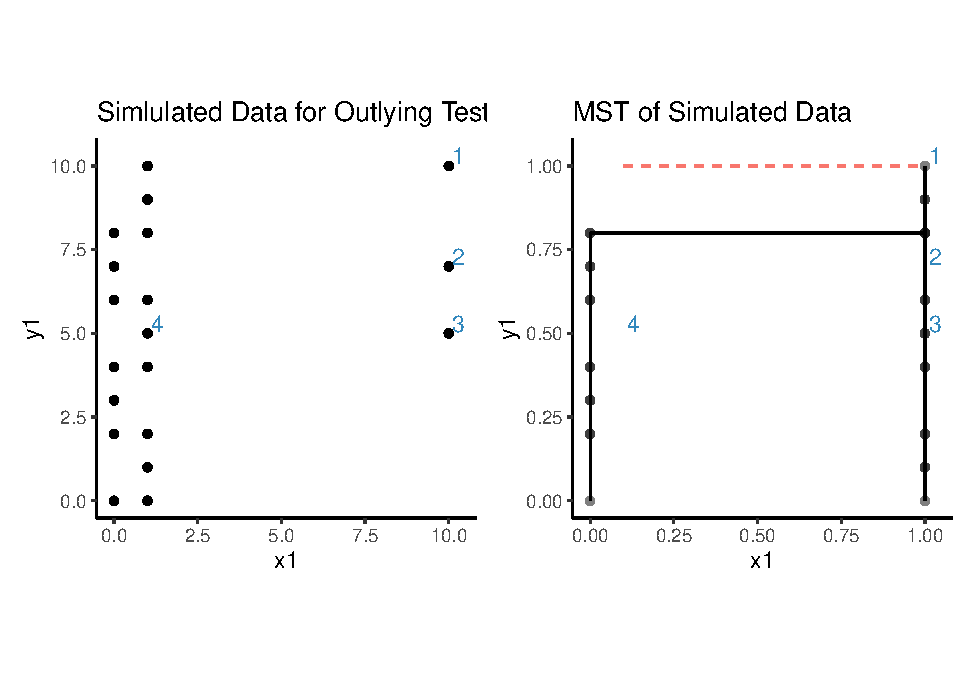
\includegraphics[width=1\linewidth]{mason-lee-laa-cook_files/figure-latex/outlying-test-plot-1} \caption[Plot of simulated data used for testing the outlying scagnostic]{Plot of simulated data used for testing the outlying scagnostic. The left plot shows the raw data, while the right plot presents the MST generated on that data. When we created the test we expected the red dashed line to be in the MST, but instead the black line that connects points 3 and 4 is. If the red edge is in the MST rather than the black edge, the outlying value on this plot is much higher.}\label{fig:outlying-test-plot}
\end{figure}
\end{Schunk}

\hypertarget{examples}{%
\section{Examples}\label{examples}}

\hypertarget{aflw-player-statistics}{%
\subsection{AFLW player statistics}\label{aflw-player-statistics}}

The Australian Football League Women's (AFLW) is the national
semi-professional Australia Rules football league for female players.
Here we will analyse data sourced from the official AFL website with
information on the 2020 season, in which the league had 14 teams and
1932 players. These variables are recorded per player per game, so the
stats are averaged for each player over the course of the season. The
description of each statistic in the data set can be found in the
appendix A1. There are 68 variables, 33 of which are numeric. The the
others are categorical, e.g.~players names or match ids, and they would
not be used in scagnostic calculations. This means there are 528
possible scatterplots, significantly more than a single person could
view and analyse themselves and so we use scagnostics to identify which
pairwise plots might be interesting to examine.

Figure \ref{fig:AFLW-scatters-static} displays five scatter plots (Plots
1 to 5 in the figure) that were identified as interesting due to having
a particularly high or low value on a scagnostic, or some unusual
combination of two or more scagnostics. In addition to these five, there
is a 6th plot (Plot 6 in the figure) that is included to display what a
middling value on almost all of the scagnostics looks like. Most scatter
plots score middling values on the scagnostics, so Plot 6 is also a good
indication of what we would look at if we picked variables to plot
ourselves with no intuition. The visual structure that changes
significantly between Plots 1 to 5, and the lack of interesting visual
features in Plot 6, shows the benefit of using scagnostics in the early
stages of exploratory data analysis.

\begin{Schunk}
\begin{figure}

{\centering 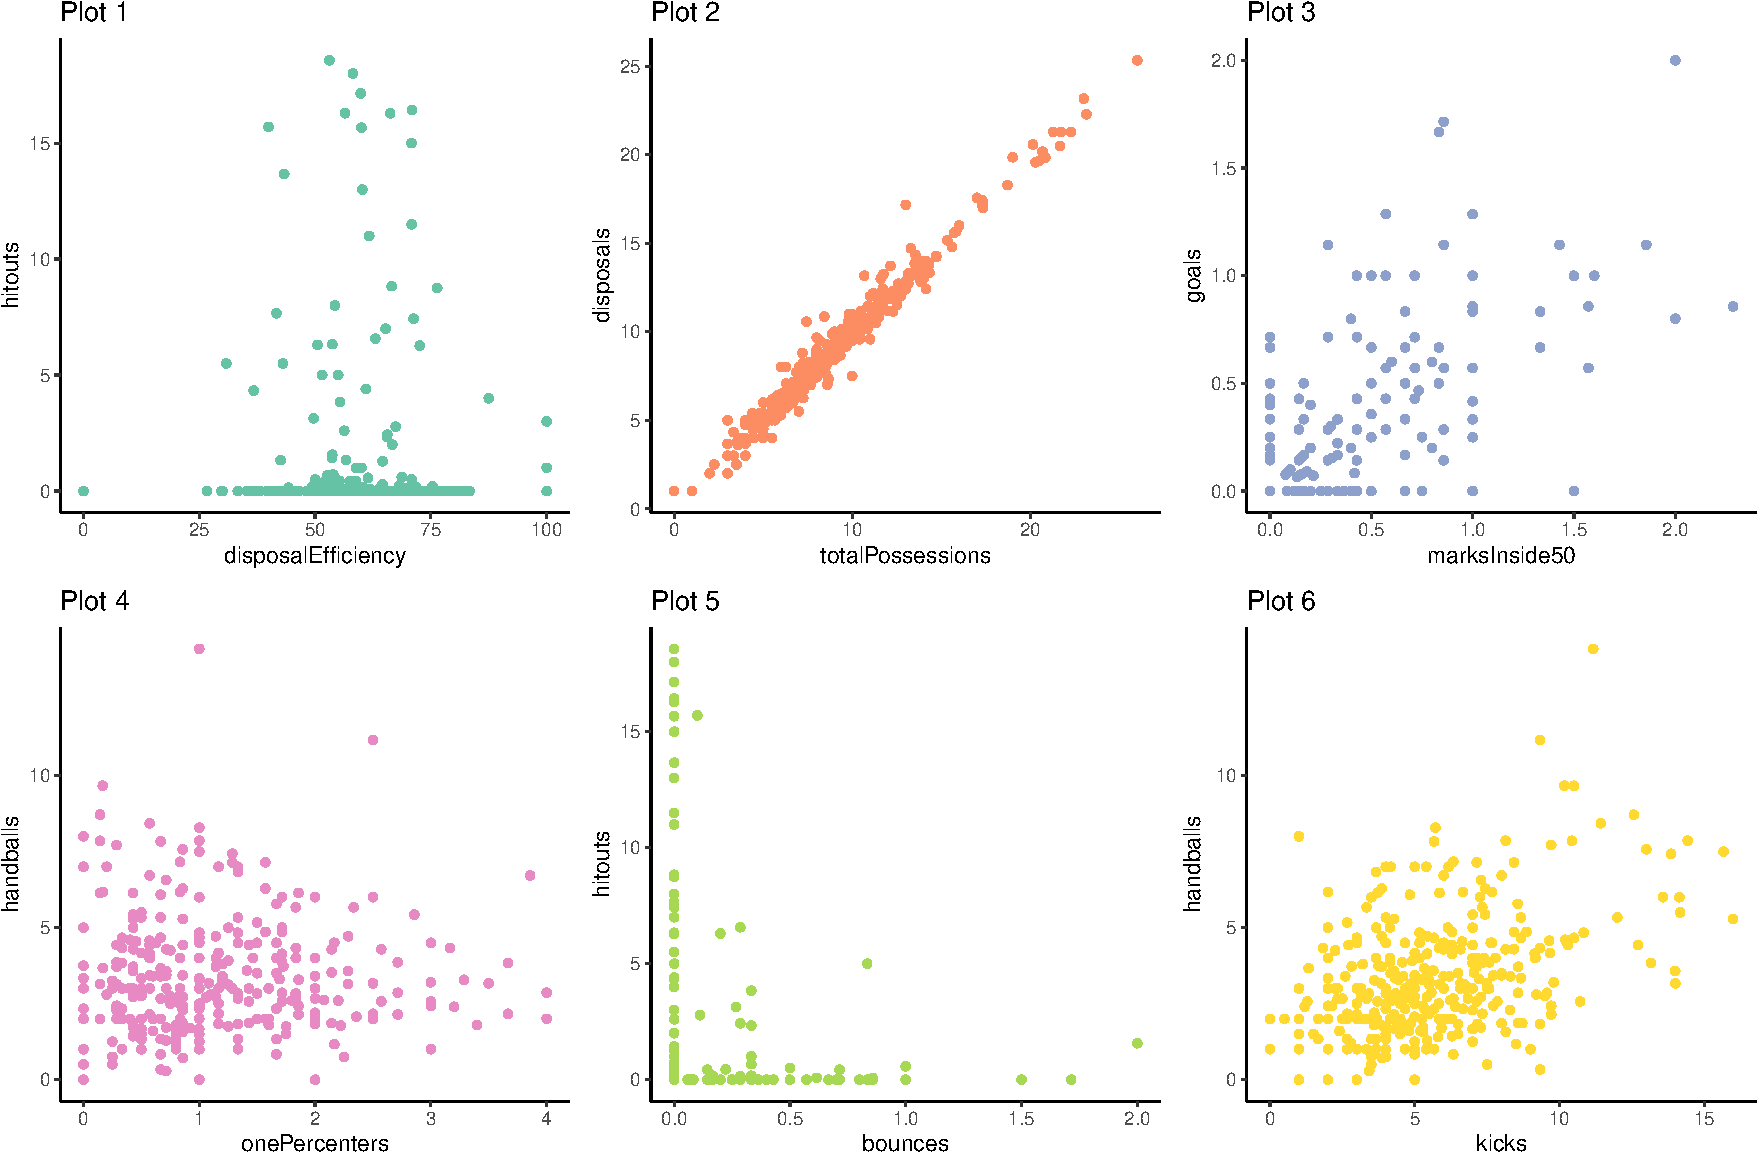
\includegraphics[width=1\linewidth]{mason-lee-laa-cook_files/figure-latex/AFLW-scatters-static-1} 

}

\caption[Six AFLW sport statistics scatter plots that were identified as identified as interesting by the scagnostics]{Six AFLW sport statistics scatter plots that were identified as identified as interesting by the scagnostics. Plots 1 to 5 had unique values on some combination of the scagnostics, Plot 6 had middling values on all measures. There is a clear difference in structure between these plots indicating the scagnostics ability to identify interesting visual features.}\label{fig:AFLW-scatters-static}
\end{figure}
\end{Schunk}

The best way to identify interesting scatter plots is to construct a
large interactive SPLOM of the scagnostic values,each point representing
a scatter plot in the data set. This is how Plots 1 to 6 were
identified, but for the sake of space, we are only going to show the
scatter plots of the SPLOM that led to the selection of Plots 1, 2, and
5.

Figure \ref{fig:threeplot-static} displays Plot 1, Plot2 and Plot 5
beneath the scatter plot of the scagnostics SPLOM that was used to
identify it as interesting. Plot 1 was identified as interesting as it
returned high values on both outlying and skewed. Intuitively, this
would indicate that even after removing outliers, the data was still
disproportionately spread out. This visual feature can be seen very
clearly in Plot 1. Plot 2 scored very highly on all the association
measures, which indicates a strong relationship between the two
variables. The three association measures typically have strong
correlation and scatter plots that stay within the large mass in the
center have a linear relation, those that don't often have a non-linear
relationship. The splines vs dcor plot tells us that there is a strong
linear relationship between total possessions and disposals. Total
possessions is the number of times the player has the ball and disposals
is the number of times the player gets rid of the ball legally, so the
strong linear relation indicates the level of play, and tells us few
mistakes are made in a professional league. Plot 5 is an excellent
example in what new information we can learn from a unique plot
identified with scagnostics. This plot is high on striated2 and moderate
to low on outlying, telling us most of the points will be at straight or
right angles and a little spread out. Hitouts measure the number of
times the player punches the ball after the referee throws it back into
play, and are typically done by tall players. Bounces have to be done
while running, and are typically done by fast players. The L-shape of
the plot tells us that players who do one very rarely perform the other,
so the tallest player in AFL is rarely the fastest. The skewed spread
along both of the statistics tells us these are both specialised skills.
These plots provide a clear example of the unique information gained
using scagnostics as a tool in exploratory data analysis.

\begin{Schunk}
\begin{figure}

{\centering 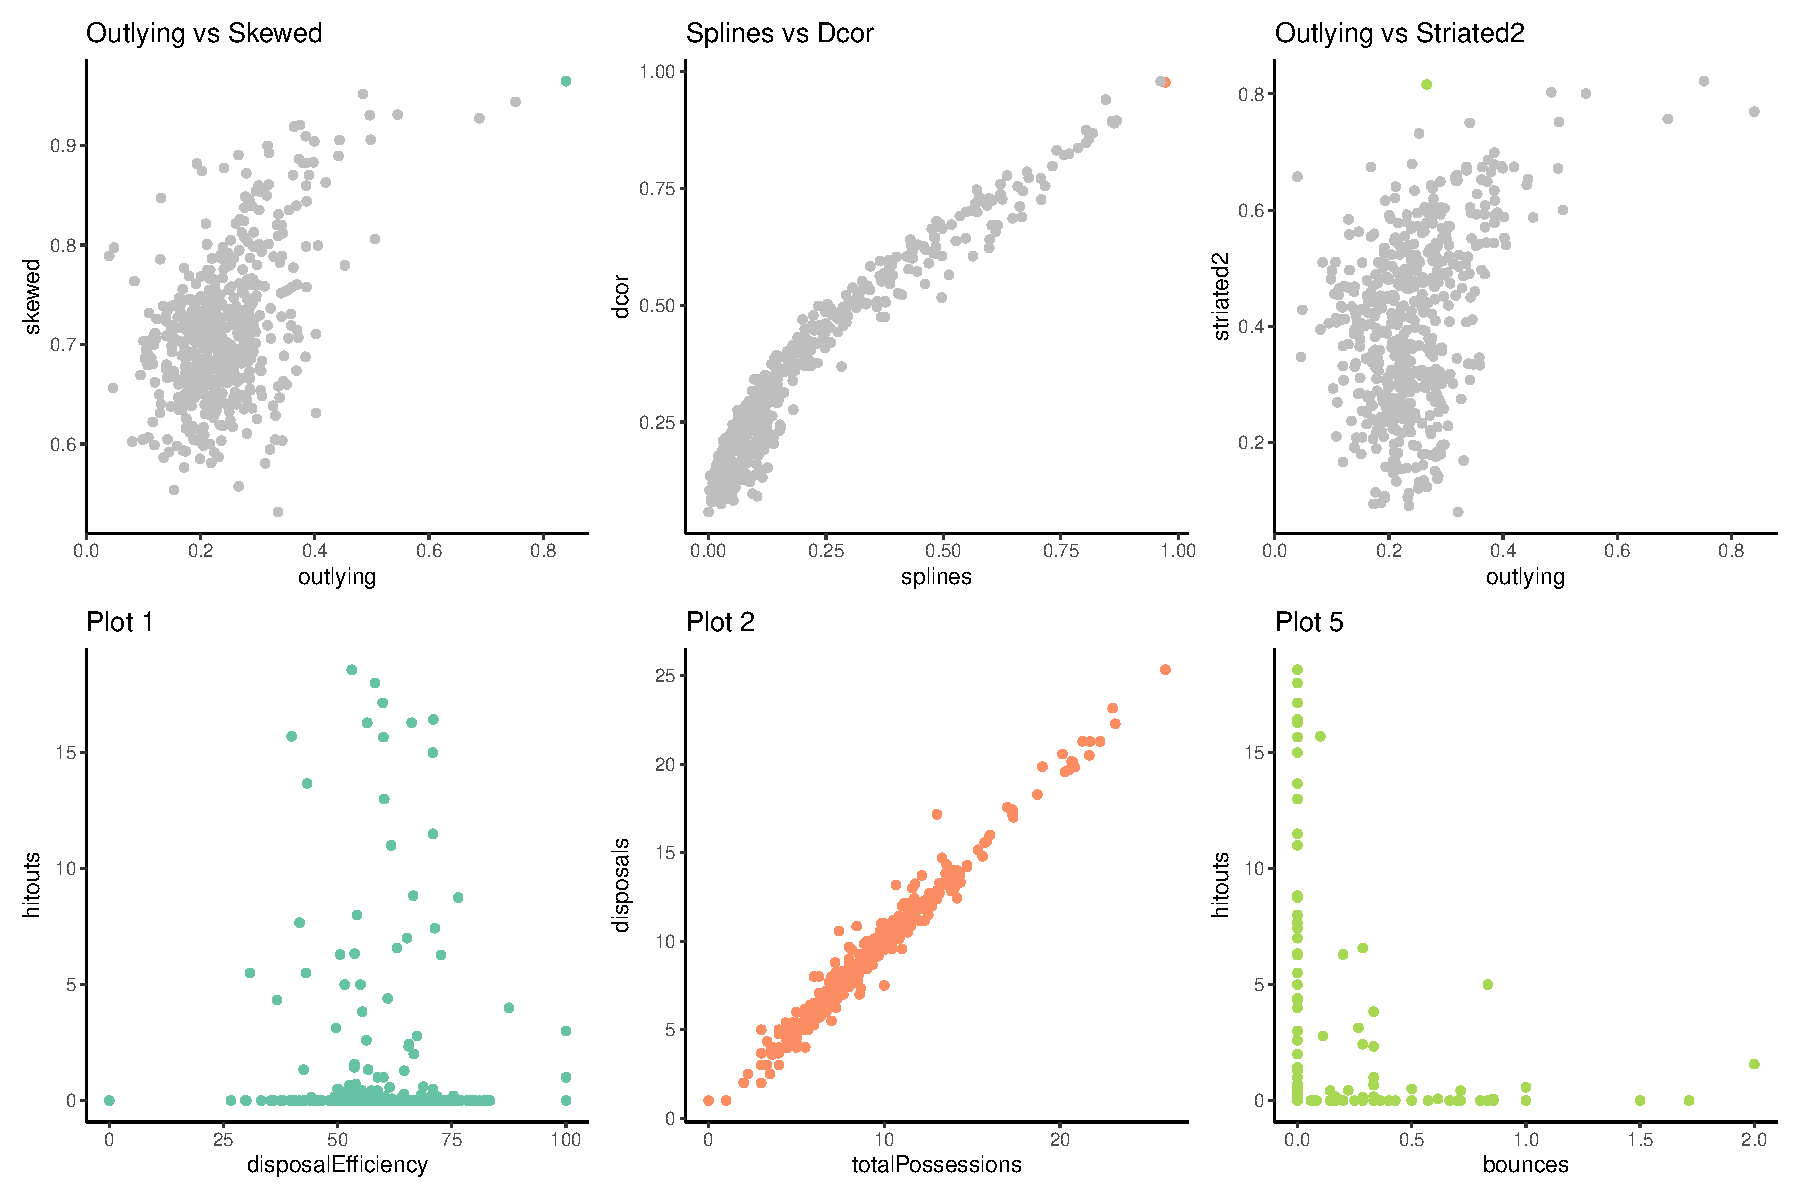
\includegraphics[width=1\linewidth]{mason-lee-laa-cook_files/figure-latex/threeplot-static-1} 

}

\caption[Three plots that were identified as interesting with the scagnostic scatter plot used to identify it]{Three plots that were identified as interesting with the scagnostic scatter plot used to identify it. Each scatter plot of AFLW data is displayed below a plot of the two scagnostic measures it stood out on. One of the most useful ways to identify plots is through scatter plots of the scagnostics.}\label{fig:threeplot-static}
\end{figure}
\end{Schunk}

\hypertarget{non-linear-shapes-in-black-hole-mergers}{%
\subsection{Non-linear shapes in black hole
mergers}\label{non-linear-shapes-in-black-hole-mergers}}

Physics data often contains multiple variables with highly non-linear or
clustered pairwise relationships, which makes this type of data ideal
for displaying the applications of splines and clumpy2; two scagnostics
that's uses were not particularly visible in the AFLW example. Here we
will use scagnostics to explore data that comes from a simulation of a
model describing a binary black hole (BBH) merger event. The data
contains 13 variables that describe the BBH event, and each point is a
posterior sample that could describe the event. As the data describes a
complicated physics phenomena, brief details of the variables will be
left to appendix A2 as a deeper understanding requires a non-trivial
amount of knowledge in physics. Therefore, we will focus on the types of
patterns observed rather than an interpretation of these patterns.

The full data file contains 9998 posterior samples, and with such a
large number of observations, the scagnostics cannot be computed within
a reasonable time frame without the assistance of binning. For our
purpose a much smaller sample is sufficient, and we randomly sample 200
observations before computing the scagnostics. Since the size of the
dataset is small enough, looking at the complete SPLOM of the data is
still feasible, and could be used to identify several interesting
scatterplots. We will omit the SPLOM here, however it allows us to see
the presence of non-linear and non-functional relations between pairs of
variables that we except the scagnostics to pick out. For this reason,
we will focus on scatter plots that have low convex values and high
skinny values, a significant difference in their splines and dcor
values, or stand out on the clumpy2 measure, as these three qualities
indicate the presence of non-linear or clustered relationship.

\begin{Schunk}
\begin{figure}
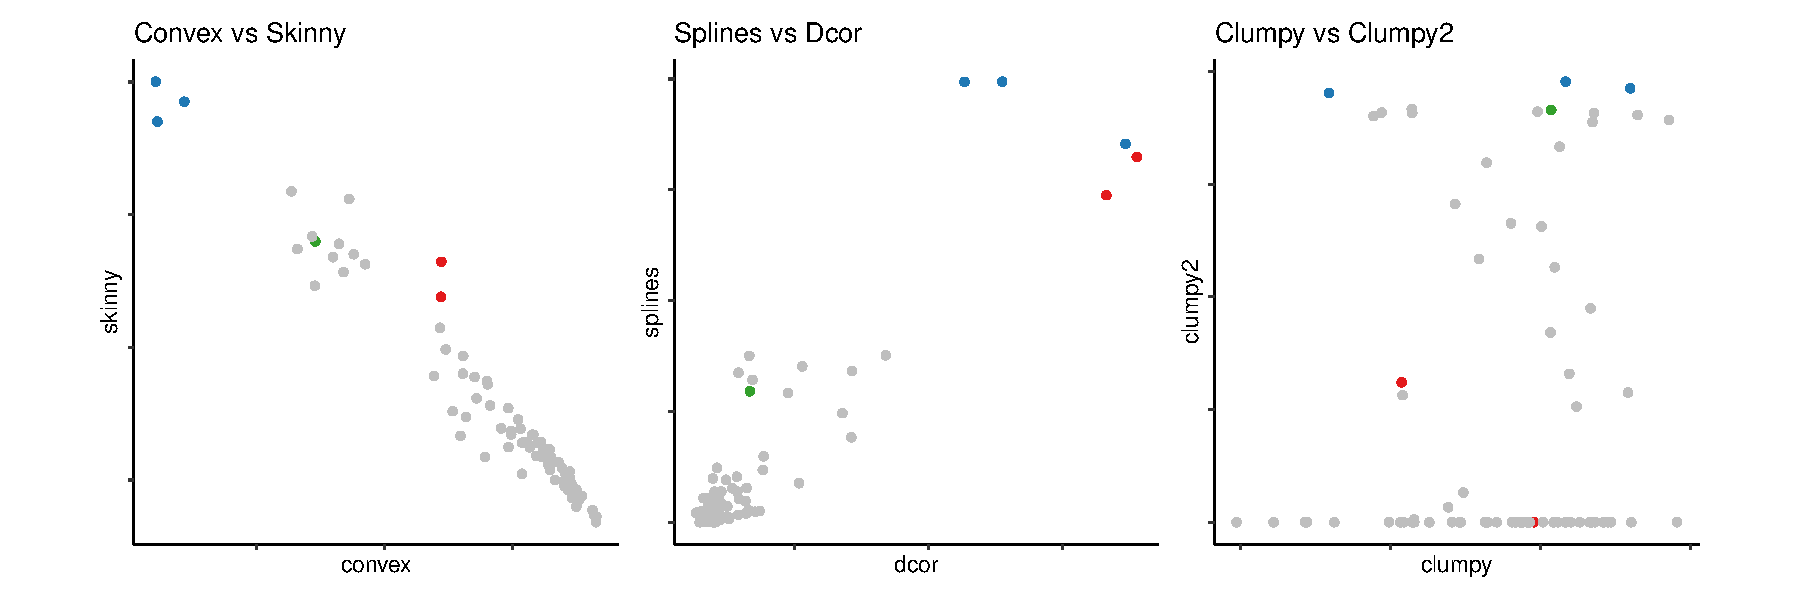
\includegraphics[width=1\linewidth]{mason-lee-laa-cook_files/figure-latex/bbh-scags-static-1} \caption[Selected pairs of scagnostics computed for the black hole mergers data]{Selected pairs of scagnostics computed for the black hole mergers data. The coloured points in these plots align with the plot colours of Figure 11. Groups of parameter combinations can be seen to stand out in the left plot (high on skinny and low on convex) and in the middle plot (high on both dcor and splines). The plot on the right shows clumpy vs clumpy2, where we can see a large impact of the correction. }\label{fig:bbh-scags-static}
\end{figure}
\end{Schunk}

Figure \ref{fig:bbh-scags-static} shows scatter plots of the relevant
scagnostics measures; outlying, skinny, splines, dcor, clumpy, and
clumpy2. On the left plot we see three points with very low values of
the convex measure and high values of skinny. This combination of
variables indicates some narrow shape and turns out to correspond to all
the possible combinations containing the variables time, ra and dec. The
corresponding scatterplots are shown in the upper row of Figure
\ref{fig:blackholes}. This pattern arises because the location of an
event observed from gravitational waves can only be localized when using
a network of three detectors (as described in \citet{gwtriang}), and
observations with one or two detectors will result in a degeneracy
between the location in the sky (parametrized by ra and dec) and the
time of the event (time). It will lead to the observed pattern of a
broken ring in this three dimensional space, thus inducing both
non-linear dependence and clustering in the posterior sample.

These three variables also stand out in the middle plot of Figure
\ref{fig:bbh-scags-static}, where the two plots involving ra that have a
non-linear but functional relation have a somewhat higher values in the
splines measure compared to dcor. On the other hand dec vs time does not
exhibit a functional relation, and consequently gets a higher dcor score
compared to splines (with both measures still taking large values). This
also happens for two other combinations: m1 vs m2 and chi\_p vs
chi\_tot, which are shown in the bottom row (left and middle) of Figure
\ref{fig:blackholes}. We see that both these combinations show noisy
linear relations.

Another interesting aspect of this dataset is that there are several
combinations that lead to visible separations between groups of points.
This makes it an ideal test case for our new implementation of clumpy2.
The right plot in Figure \ref{fig:bbh-scags-static} shows clumpy vs
clumpy2, and reveals large differences between the two measures. In
particular there are many combinations without visible clustering, that
still score high on clumpy, but where clumpy2 is zero. On the other hand
we can see that there are several combinations that do lead to visible
separation between groups that stand out in terms of clumpy2, but not
the original clumpy. One example is time vs alpha, shown in the bottom
right plot of Figure \ref{fig:blackholes}.

\begin{Schunk}
\begin{figure}
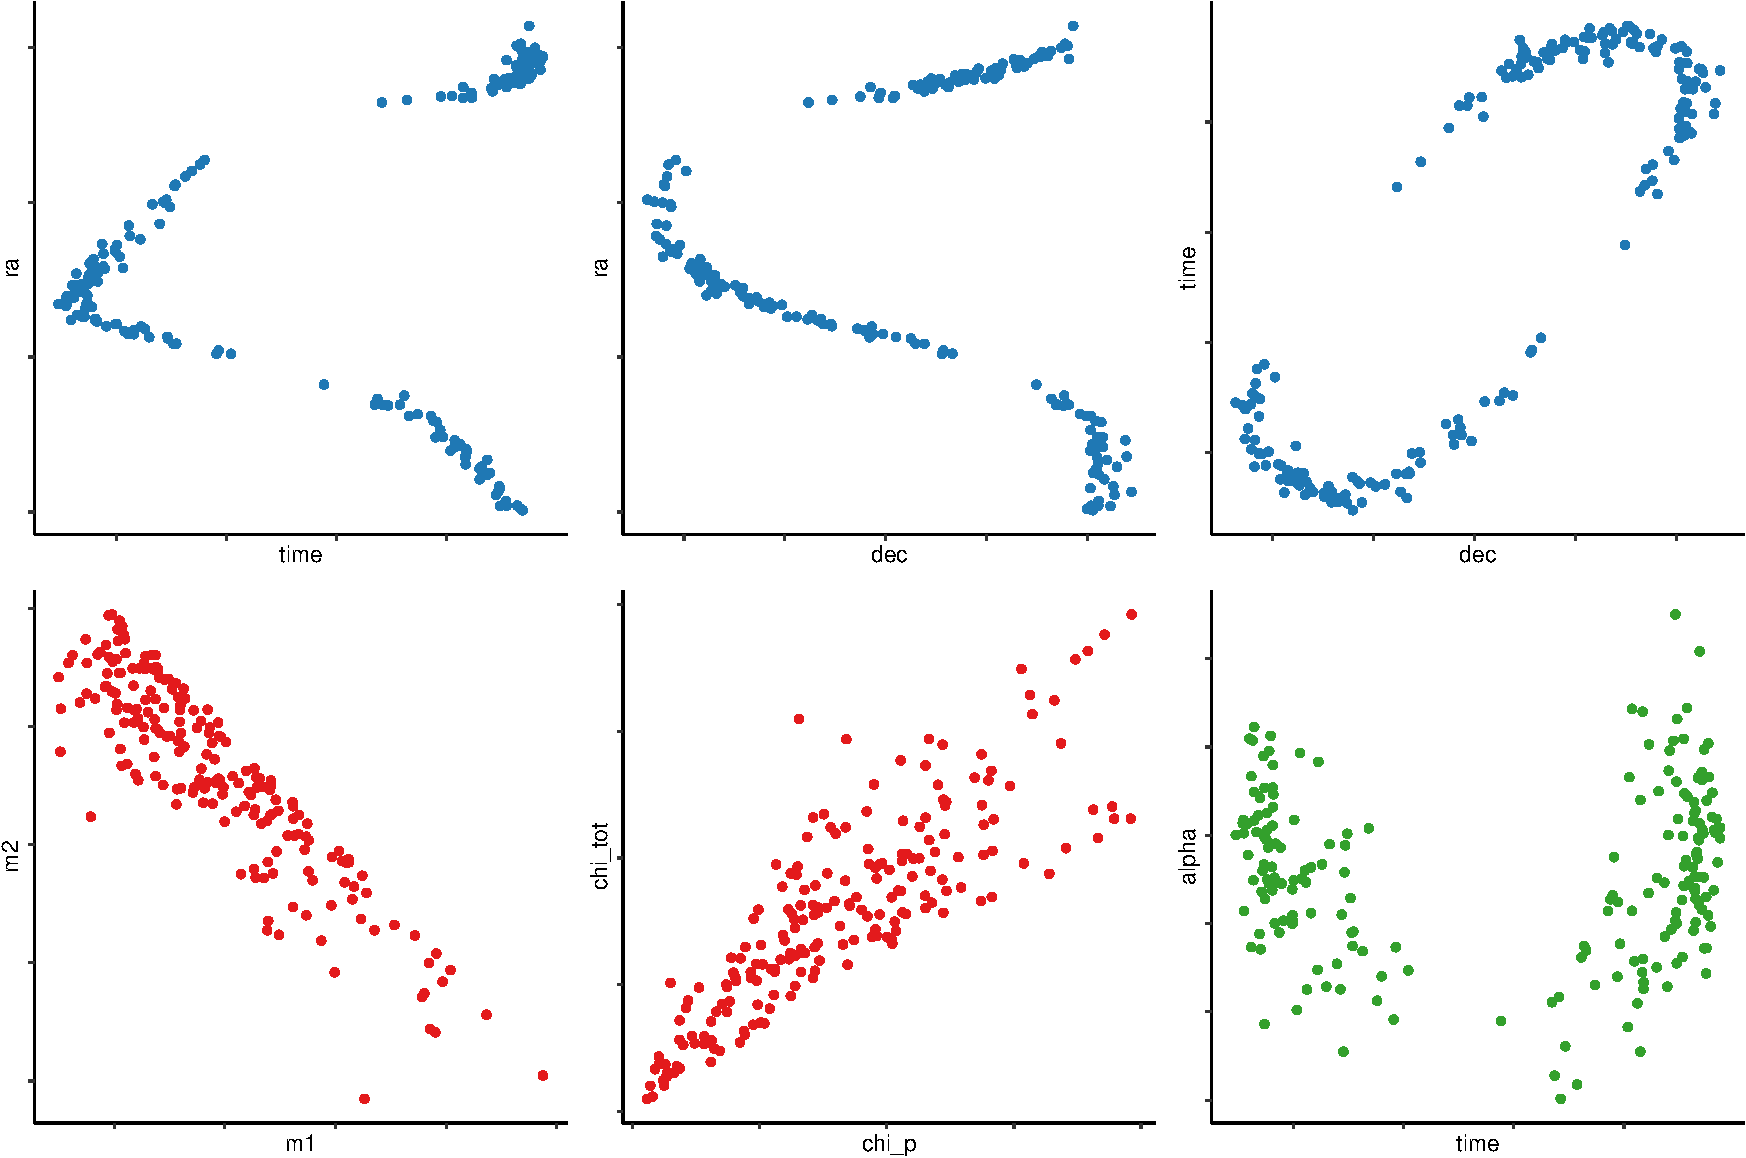
\includegraphics[width=1\linewidth]{mason-lee-laa-cook_files/figure-latex/blackholes-1} \caption[Features in the BBH data that stand out on several of the scagnostics measures (convey, skinny, splines and dcor), showing strong relations between variables including non-linear and non-functional dependencies]{Features in the BBH data that stand out on several of the scagnostics measures (convey, skinny, splines and dcor), showing strong relations between variables including non-linear and non-functional dependencies. The colour of these point align with the plots position in the plots of Figure 10. The final example (time vs alpha) is expected to take high values in clumpy, but only stands out on the corrected clumpy2.}\label{fig:blackholes}
\end{figure}
\end{Schunk}

\hypertarget{shape-differences-between-groups}{%
\subsection{Shape differences between
groups}\label{shape-differences-between-groups}}

A potential application of scagnostics is to detect shape differences
between groups, in contrast to the more common classification by
differences in means or gaps. A difference in shape corresponds to
different covariance patterns between groups. A way to think about this
is contrasting linear discriminant analysis (LDA) with quadratic
discriminant analysis (QDA). LDA assumes the distribution of each group
is multivariate normal with the same means and the same variance. The
classification boundary is planar at a maximal distance from each groups
mean, with orientation of the plane determined by the pooled
variance-covariance matrix. QDA similarly assumes the distribution of
each group is normal, but relaxes the assumption of equal
variance-covariance. The boundary between groups has a quadratic form.
So from this, it can be seen that QDA is more flexible than LDA as it
accommodates shape differences. However shape differences are
constrained to be elliptical based on the assumption of normality.
Scagnostics could be utilised to broadly identify irregular shape
differences between groups.

To illustrate this analysis, we consider comparing two sets of time
series, described by their features, such as trend, spikiness, acf,
using scagnostics. The goal of the comparison is to compare shapes, not
necessarily centres of groups as might be done in LDA or other machine
learning methods. The two groups chosen for comparison are macroeconomic
and microeconomic series. The data for 100 series of each type is pulled
from the self-organizing database of time-series data \citep{sots},
using the \texttt{compenginets} R package \citep{compenginets}. Since
the time series are different lengths, each is described by a set of
time series features \citep[chapter 4 of][]{fpp} using the
\texttt{feasts} R package \citep{feasts}.

To keep the illustration simple, a small set of seven features is
examined. Table \ref{tab:scagsmacmic-pdf} tabulates pairs of features
that have the biggest difference between groups across a range of
scagnostics. Plotting a handful of these in (Figure
\ref{fig:timeseries}), we can see the differences in shape that the
scagnostics have identified. For example, the scagnostic \emph{skewed}
selects the pair of features, curvature and trend strength, and reveals
a shape difference in these features between macroeconomic and
microeconomic time series (middle plot). Macroeconomic series tend to
have moderate curvature and varied trend, while microeconomic series
tend to have strong trends and varied curvature. These feature
differences that are identified in the scagnostic can be seen in the
time series themselves in Figure \ref{fig:tsplots}. We can see from this
example, and the other comparisons in the plot, that the scagnostics
have identified a differences in shape that would not have been apparent
from only examining mean differences between groups. Other shape
differences can be read from the other pairs of features (left and right
plots).

While we have shown that the scagnostics succeed in identifying
difference in shapes between groups, this does not automatically
transfer to a classification technique. Utilising the scagnostics
ability to identify between group shape differences is an early step in
using them for classification. It is not uncommon for supervised
learning methods to be born from unsupervised learning methods. For
example, principal component analysis (PCA), an unsupervised learning
method, transforms a data set by making linear combinations of the
variables in the direction of most variance. Performing this linear
transformation wile also trying to explain the variance in a response
variable is a supervised version of PCA known as principal component
regression. However, despite its promise, developing a classification
technique based on scagnostics is beyond the scope of this paper.

\begin{Schunk}
\begin{table}

\caption{\label{tab:scagsmacmic-pdf}Pairs of time series features that have large differences between macroeconomic and microeconomic series on a range of scagnostics.}
\centering
\begin{tabular}[t]{lllrrr}
\toprule
Variable 1 & Variable 2 & Scagnostic & Macro Value & Micro Value & Difference\\
\midrule
acf1 & trend strength & clumpy2 & 0.83 & 0.00 & 0.83\\
longest flat spot & trend strength & convex & 0.12 & 0.62 & 0.50\\
pacf5 & diff1 acf1 & outlying & 0.32 & 0.71 & 0.39\\
curvature & trend strength & skewed & 0.65 & 0.84 & 0.19\\
longest flat spot & trend strength & skinny & 0.64 & 0.37 & 0.27\\
\addlinespace
acf1 & trend strength & sparse & 0.04 & 0.11 & 0.07\\
pacf5 & acf1 & splines & 0.88 & 0.00 & 0.88\\
longest flat spot & diff1 acf1 & striated2 & 0.13 & 0.06 & 0.06\\
diff1 acf1 & trend strength & stringy & 0.84 & 0.73 & 0.11\\
\bottomrule
\end{tabular}
\end{table}

\end{Schunk}

\begin{Schunk}
\begin{figure}
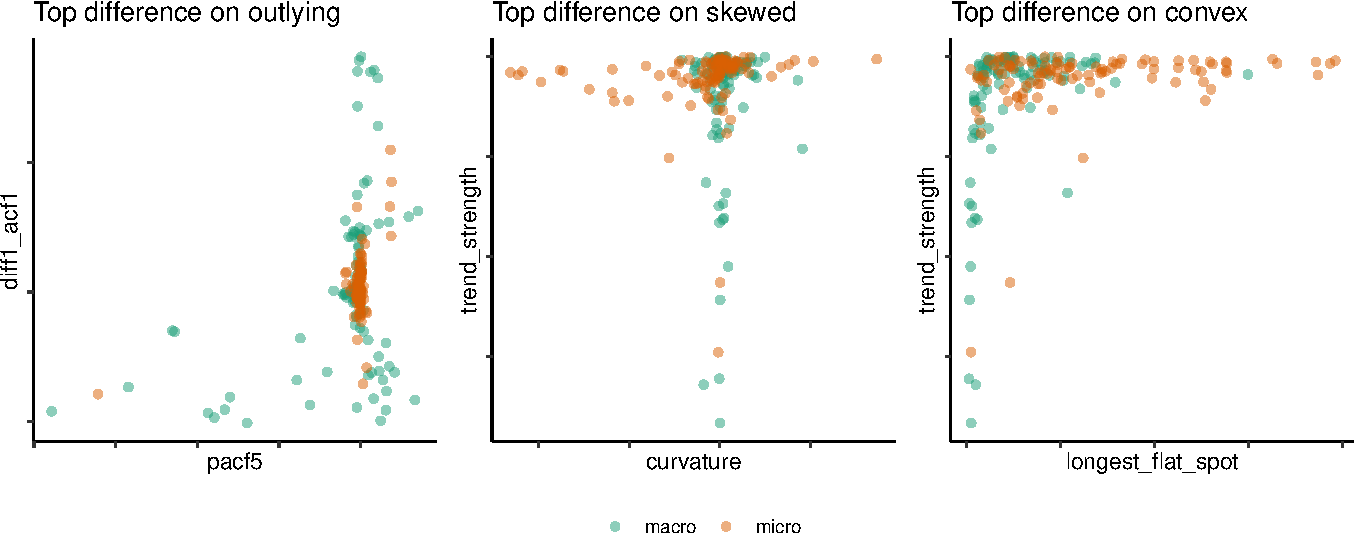
\includegraphics[width=1\linewidth]{mason-lee-laa-cook_files/figure-latex/timeseries-1} \caption[Interesting differences in the visual features of two groups of time series can be detected by scagnostics]{Interesting differences in the visual features of two groups of time series can be detected by scagnostics. The three plots represent the variable pairs that maximised the differences between outlying (left), skewed (middle) and convex (right). While these distributions may have overlapping means, their differencs in shape have been identified by the scagnostics.}\label{fig:timeseries}
\end{figure}
\end{Schunk}

\begin{Schunk}
\begin{figure}
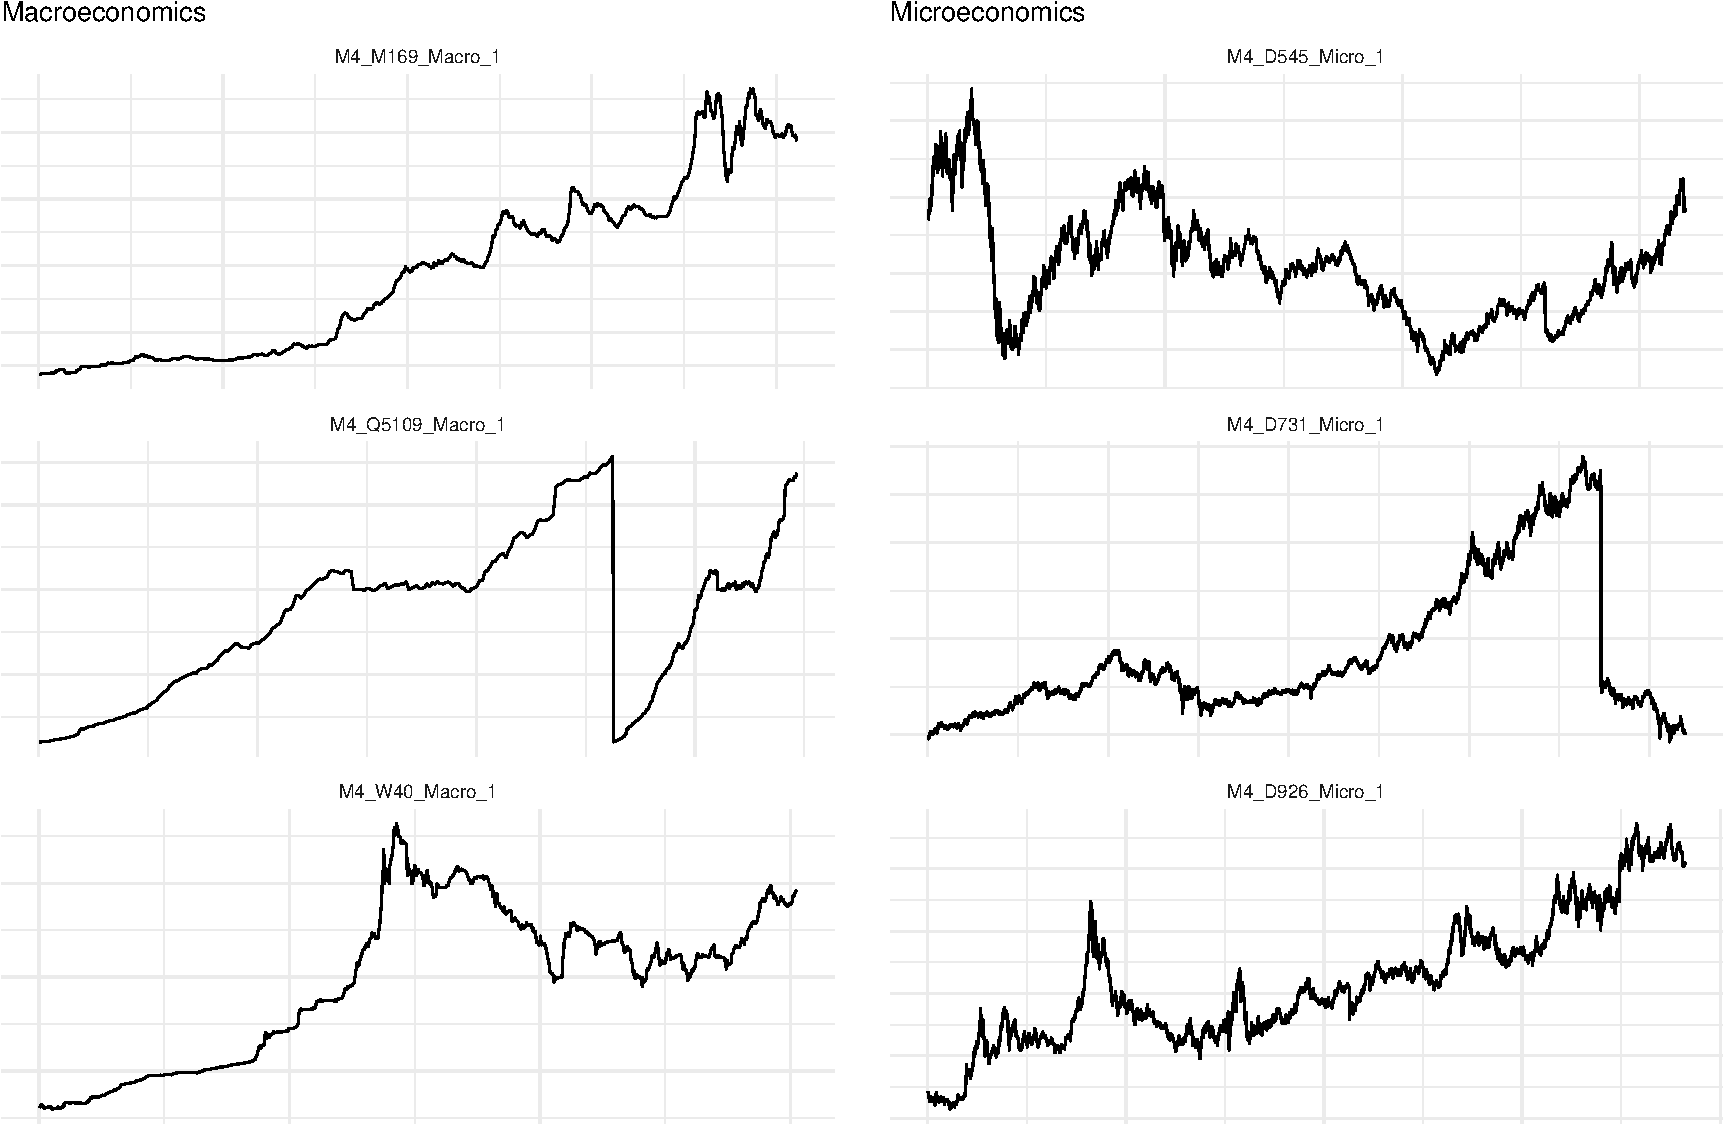
\includegraphics[width=1\linewidth]{mason-lee-laa-cook_files/figure-latex/tsplots-1} \caption[Selection of three series from the 100 of each of two groups, macroeconomics and microeconomics]{Selection of three series from the 100 of each of two groups, macroeconomics and microeconomics. The difference between the groups appears to be primarily in the jagginess of the two series, which a little surprisingly, is captured by the time series features curvature and trend strength. The way that trend strength is calculated, on closer inspection, could lead to describing jagginess.}\label{fig:tsplots}
\end{figure}
\end{Schunk}

\hypertarget{processing-and-describing-data-with-many-variables}{%
\subsection{Processing and describing data with many
variables}\label{processing-and-describing-data-with-many-variables}}

The World Bank delivers a lot of development indicators (WBI)
\citep{WBI}, for many countries and multiple years. The sheer volume of
indicators, in addition to the substantial number of missing values,
presents a barrier to analysis. This is a good example where scagnostics
can be used to identify pairs of indicators with interesting
relationships, and efficiently handle missing values on a pairwise
basis.

The downloaded data uses indicators from 2018 and after some
pre-processing to remove variables or countries which have mostly
missing values, there are 20 indicators (variables) and 79 countries in
our data set. The variable names are somewhat cryptic, and their
descriptions are left to the appendix A3. The scagnostics will be
calculated on this pairwise complete data, allowing for a few sporadic
missings.

Figure \ref{fig:wbistatic} (left plot) shows a summary of the top
scagnostic value for each pair of variables, that is, only the highest
scagnostic value for each pair of variables is saved. This is displayed
as a vertically-oriented side-by-side dotplot. For the WBI data, the
pairs of variables are producing mostly high values on stringy, skewed,
convex and outlying, while the scagnostics clumpy2, striated2, and
skinny are only the highest for a single pair of variables. In addition,
missing from the plot but not the calculations is that splines was not
the highest for any pair of variables in the data set.

This tells us that in the WBI data, the relationships between variables
is dominated by outliers (as noted by the high values on the outlying
scagnostic, and to some extent also skewed and stringy), and no
relationship (given bu the high values on convex). Scagnostics might be
useful for obtaining alternative descriptive summaries of data with many
variables. We can visualise some individual scatter plots to check this
shape summary. The middle plot of Figure \ref{fig:wbistatic} show the
pair of variables where clumpy2 has the highest value, a plot that does
not stand out as ``clumpy''. The right plot in the figure is one of many
in which convex has the highest value (a plot with no relationship).
This helps us confirm what the shape summary tells us that the data,
that most variable pairs have no relationships or clustering.

\begin{Schunk}
\begin{figure}
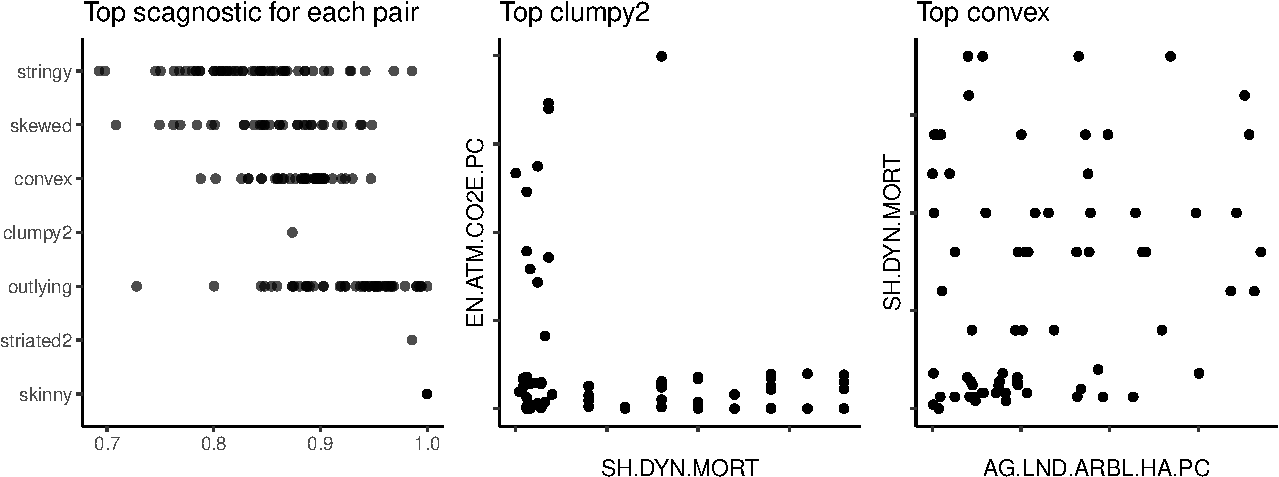
\includegraphics[width=1\linewidth]{mason-lee-laa-cook_files/figure-latex/wbistatic-1} \caption[Using scagnostics to explore the variety of relationships present in the WBI data]{Using scagnostics to explore the variety of relationships present in the WBI data. The side-by-side dotplot (left) shows one point for each pair of variables, with its highest scagnostic value among all scagnostics calculated. Most of the pairs of indicators exhibit outliers, skewed, stringy or convex. There is one pair that has clumpy as the highest value. The plots, middle and right, show the pair of variables with highest value on clumpy2 and convex, respectively.}\label{fig:wbistatic}
\end{figure}
\end{Schunk}

\hypertarget{conclusion}{%
\section{Conclusion}\label{conclusion}}

Scagnostics are a useful tool to identify the visual features in scatter
plots. Building upon previous work, a new set of scagnostics, that do
not require binning, have been implemented and made available in the
\emph{cassowaryr} R package. Explanations of the scagnostics and the
details of the package were provided, along with four examples of use;
AFLW, black hole mergers, time series and WBI. AFLW shows the general
use of the \emph{cassowaryr} package, and how to use scagnostics to find
unique scatter plots. In this example, we also showed that looking at
specific pairwise scatter plots can give us valuable information about a
data set by interpreting the \emph{hitouts vs bounces} scatter plot in
Figure \ref{fig:threeplot-static}. Using simulated data of a black hole
merger event, we then displayed the packages ability to identify
pairwise non-linear relationships with convex, skinny, splines, and
dcor, as well as the improvement clumpy2 made in identifying clustering.
The time series example displayed how the scagnostics could be used for
classification, illustrating how macro and micro economic time series
can be distinguished by different shapes in feature sets. In the last
example, the scagnostics applied to the WBI show that they can be used
to produce an overall \emph{shape summary} of a data set.

There are a number of different directions to build upon this research.
The original scagnostics used binning as a pre-processing step. This
will be useful to include to improve speed of calculations with larger
sample sizes. The scale of the scagnostics is the same, ranging from 0
through 1, which allows comparison across scagnostics. However, the
distribution may be different. In the WBI example, describing the
overall shape of the data requires the assumption that the scagnostics
are all uniformly distributed from 0 to 1. However, as some of our
results suggest, and also as seen in the visual table of the features
scatter plots (Figure \ref{fig:visual-table}), this may not be the case.
It would be a substantial task to identify the distributions of the
scagnostics, and make adjustments to transform to uniform distributions.
The scagnostics would need to be studied using large volumes of data to
capture their performance over all possible data shapes. Scagnostics
could be developed further into a classification technique that
identifies shape differences between groups. While the time series
example shows that scagnostics can identify shape differences between
groups, extending this observation to a stand alone classification
technique is outside the scope of this paper but is still a possible
area of future research. \citet{hidscags} showed that scagnostics can be
used to identify hidden structure in pairwise plots after
transformations such as a log of the original data. This offers a
natural extension for the scagnostics that could be added to the
\texttt{cassowaryr} package. Finally, scagnostics could be used to
examine scatterplots generated by a 2D projection of multiple variables,
as in the projection pursuit guided tour in the \texttt{tourr} package.
The primary barrier in past use has been in optimisation, because the
scagnostic values over smooth sequences of projections can be noisy.
This would need to be checked for the new scagnostic measures is order
to use them for projection pursuit.

The implementation in R also makes it easy to expand the scagnostics
collection and develop new measures. Other researchers can easily expand
the package with new measures or enhance the current code because the
software is openly available on GitHub, encouraging contributions from
the broader community.

\hypertarget{acknowledgements}{%
\section{Acknowledgements}\label{acknowledgements}}

This article is created using \CRANpkg{knitr} \citep{knitr} and
\CRANpkg{rmarkdown} \citep{rmarkdown} in R. The source code for
reproducing this paper can be found at:
\url{https://github.com/harriet-mason/paper-cassowaryr}.

\hypertarget{appendix}{%
\section{Appendix}\label{appendix}}

\hypertarget{a1-aflw-data-dictionary}{%
\subsection{A1: AFLW Data Dictionary}\label{a1-aflw-data-dictionary}}

\begin{itemize}
\tightlist
\item
  \emph{timeOnGroundPercentage}: percentage of the game the player was
  on the field.
\item
  \emph{goals}: the 6 points a team gets when the kick the ball between
  the two big posts.
\item
  \emph{behinds}: the 1 point a team gets when they kick the ball
  between the big post and small post.
\item
  \emph{kicks}: number of kicks done by the player in this game.
\item
  \emph{handballs}: number of handballs does by the player in the game.
\item
  \emph{disposals}: the number kicks and handballs a player has.
\item
  \emph{marks}: total number of marks in the game (the ball travels more
  than 15m and the player catches it without another player touching it
  or it hitting the ground).
\item
  \emph{bounces}: the number of times a player bounced the ball in a
  game. A player must bounce the ball if they travel more than 15m and
  they can only bounce the ball once.
\item
  \emph{tackles}: Number of tackles performed by the player.
\item
  \emph{contestedPossessions}: the number of disposals a player has
  under pressure, i.e if a player is getting tackled and the get a
  handball or kick out of the scuffle.
\item
  \emph{uncontestedPossessions}: the number of disposals a player has
  under no pressure where they have space and time to get rid of the
  ball.
\item
  \emph{totalPossessions}: The total number of time the player has the
  ball.
\item
  \emph{inside50s}: the number of times the player has the ball within
  the 50m arc around the opponents goals.
\item
  \emph{marksInside50}: the number of marks a player gets within the 50m
  arc around the opponents goals.
\item
  \emph{contestedMarks}: the number of marks a player has under
  pressure.
\item
  \emph{hitouts}: this is how many times a player or team taps or
  punching the ball from a stoppage.
\item
  \emph{onePercenters}: all the things a player can do without
  registering a disposal, e.g.~Spoils (punching the ball to stop someone
  from marking it), Shepparding (blocking for a teammate), smothering.
\item
  \emph{disposalEfficiency}: a measure of how well a player disposes of
  the ball. E.g. if a player kicks or handballs to the opposition a lot,
  they will have a low disposal efficiency percentage.
\item
  \emph{clangers}: this is how many times a player or team dispose of
  the ball and it results in a turnover to the other team.
\item
  \emph{freesFor}: this player was awarded a free kick.
\item
  \emph{freesAgainst}: this player caused a free kick to be awarded to
  the other team.
\item
  \emph{dreamTeamPoints}: this is fantasy football scoring points.
\item
  \emph{rebound50s}: how many times the player exits the ball out of
  their defence 50m arc.
\item
  \emph{goalAssists}: number of times the player gave the pass
  immediately before the player that scored a goal.
\item
  \emph{goalAccuracy}: percentage ratio of the number of goals kicked to
  the number of goal attempts.
\item
  \emph{turnovers}: this players disposal caused a turnover (the ball
  touches the ground and the other team get it).
\item
  \emph{intercepts}: number of times this player intercepts the disposal
  of the other team.
\item
  \emph{tacklesInside50}: number of tackles performed by this player
  within their defence 50m arc.
\item
  \emph{shotsAtGoal}: number of total shots at goal for this player (sum
  of goals, behinds and misses).
\item
  \emph{scoreInvolvements}: number of times the player was involved in a
  passage of play leading up to a goal.
\item
  \emph{metresGained}: how far a player has been able to advance the
  ball without turning it over.
\item
  \emph{clearances.centreClearances}: this is the clearance from the
  centre bounce after a goal or at the start of a quarter.
\item
  \emph{clearances.stoppageClearances}: all the clearance from stoppages
  around the ground.
\item
  \emph{clearances.totalClearances}: how many time a player or team
  clears the ball from a stoppage or from the centre
\end{itemize}

\hypertarget{a2-black-hole-merger-data-dictionary}{%
\subsection{A2: Black Hole Merger Data
Dictionary}\label{a2-black-hole-merger-data-dictionary}}

\begin{itemize}
\tightlist
\item
  \emph{position} in the sky is characterized by three variables: ra
  (right ascension), dec (declination) and distance
\item
  \emph{time} of the event: time
\item
  \emph{mass} of the two black holes: m1, m2 (with m1 \textgreater{} m2)
\item
  \emph{spin} related properties: angles alpha, theta\_jn, chi\_tot,
  chi\_eff, chi\_p
\item
  \emph{polarisation angle}: psi
\item
  \emph{orbital phase}: phi\_jl
\end{itemize}

For a detailed description including a diagram explaining the different
angles describing the spin we refer to \citet{Smith:2016qas}.

\hypertarget{a3-world-bank-indicators-data-dictionary}{%
\subsection{A3: World Bank Indicators Data
Dictionary}\label{a3-world-bank-indicators-data-dictionary}}

\begin{itemize}
\tightlist
\item
  NV.AGR.TOTL.ZS Agriculture, value added (\% of GDP)
\item
  EN.ATM.CO2E.PC CO2 emissions (metric tons per capita)
\item
  NE.EXP.GNFS.ZS Exports of goods and services (\% of GDP)
\item
  DT.DOD.DECT.CD External debt stocks, total (DOD, current US\$)
\item
  SP.DYN.TFRT.IN Fertility rate, total (births per woman)
\item
  NY.GDP.MKTP.CD GDP (current US\$)
\item
  NY.GNP.MKTP.PP.CD GNI, PPP (current international \$)
  TX.VAL.TECH.MF.ZS High-technology exports (\% of manufactured exports)
\item
  SH.IMM.MEAS Immunization, measles (\% of children ages 12-23 months)
\item
  NE.IMP.GNFS.ZS Imports of goods and services (\% of GDP)
\item
  NV.IND.TOTL.ZS Industry, value added (\% of GDP)
\item
  SP.DYN.LE00.IN Life expectancy at birth, total (years)
\item
  TG.VAL.TOTL.GD.ZS Merchandise trade (\% of GDP)
\item
  MS.MIL.XPND.GD.ZS Use and distribution of these data are subject to
  Stockholm International Peace Research Institute (SIPRI) terms and
  conditions. Military expenditure (\% of GDP)
\item
  IT.CEL.SETS.P2 Mobile cellular subscriptions (per 100 people)
\item
  SH.DYN.MORT Mortality rate, under-5 (per 1,000 live births)
\item
  SP.POP.TOTL Population, total
\item
  SH.DYN.AIDS.ZS Prevalence of HIV, total (\% of population ages 15-49)
\item
  GC.TAX.TOTL.GD.ZS Tax revenue (\% of GDP)
\item
  EG.ELC.ACCS.ZS Access to electricity (\% of population)
\item
  NY.ADJ.NNTY.CD Adjusted net national income (current US\$)
\item
  SH.HIV.INCD.TL Adults (ages 15+) and children (ages 0-14) newly
  infected with HIV
\item
  AG.LND.AGRI.ZS Agricultural land (\% of land area)
\item
  ER.FSH.AQUA.MT Aquaculture production (metric tons)
\item
  AG.LND.ARBL.HA.PC Arable land (hectares per person)
\item
  MS.MIL.TOTL.TF.ZS Armed forces personnel (\% of total labor force)
\item
  FB.BNK.CAPA.ZS Bank capital to assets ratio (\%)
\item
  SE.COM.DURS Compulsory education, duration (years)
\end{itemize}

\bibliography{mason-lee-laa-cook.bib}

\address{%
Harriet Mason\\
Monash University\\%
Department of Econometrics and Business Statistics\\ Melbourne,
Australia\\
%
\url{https://www.britannica.com/animal/quokka}\\%
\textit{ORCiD: \href{https://orcid.org/0000-1721-1511-1101}{0000-1721-1511-1101}}\\%
\href{mailto:hmas0003@student.monash.edu}{\nolinkurl{hmas0003@student.monash.edu}}%
}

\address{%
Stuart Lee\\
Genentech\\%
\\
%
\url{https://stuartlee.org}\\%
\textit{ORCiD: \href{https://orcid.org/0000-0003-1179-8436}{0000-0003-1179-8436}}\\%
\href{mailto:stuart.andrew.lee@gmail.com}{\nolinkurl{stuart.andrew.lee@gmail.com}}%
}

\address{%
Ursula Laa\\
University of Natural Resources and Life Sciences\\%
Institute of Statistics\\ Vienna, Austria\\
%
\url{https://uschilaa.github.io}\\%
\textit{ORCiD: \href{https://orcid.org/0000-0002-0249-6439}{0000-0002-0249-6439}}\\%
\href{mailto:ursula.laa@boku.ac.at}{\nolinkurl{ursula.laa@boku.ac.at}}%
}

\address{%
Dianne Cook\\
Monash University\\%
Department of Econometrics and Business Statistics\\ Melbourne,
Australia\\
%
\url{https://dicook.org}\\%
\textit{ORCiD: \href{https://orcid.org/000-0002-3813-7155}{000-0002-3813-7155}}\\%
\href{mailto:dicook@monash.edu}{\nolinkurl{dicook@monash.edu}}%
}
